\documentclass{article}
\usepackage{geometry}
\usepackage{array}
\usepackage{graphicx}
\usepackage{enumitem}
\usepackage[hidelinks]{hyperref}
\usepackage{titlesec}
\usepackage{listings}
\usepackage{parskip}
\usepackage{tabularx}
\usepackage{amsmath}
\usepackage{rotating}
\usepackage{pdflscape}
\usepackage{titling}
\usepackage[UKenglish]{datetime}
\usepackage{subcaption}
\usepackage{setspace}
\graphicspath{ {images/} }


% Bibliography
\usepackage[
sorting=none,
style=ieee,
backend=biber
]{biblatex}
\addbibresource{references.bib}

% Contents page numbering depth
\setcounter{tocdepth}{2}
\setcounter{secnumdepth}{4}

% Unknown
\titleformat{\paragraph}
{\normalfont\normalsize\bfseries}{\theparagraph}{1em}{}
\titlespacing*{\paragraph}
{0pt}{3.25ex plus 1ex minus .2ex}{1.5ex plus .2ex}

%\titlespacing{\subsection}{0pt}{\parskip}{-\parskip}
\titlespacing{\subsubsection}{0pt}{\parskip}{-\parskip}
\titlespacing{\paragraph}{0pt}{\parskip}{-\parskip}
%\titlespacing{\subparagraph}{0pt}{\parskip}{-\parskip}

\renewcommand{\familydefault}{\sfdefault}

% Add page break after each section
\newcommand\sectionbreak{\clearpage}

% Set page dimensions
\geometry{a4paper, portrait, margin=2.5cm}


% Change itemize default
\def\labelitemi{--}


% Prevent horrible hyphenation
\hyphenchar\font=-1 
\righthyphenmin=62 
\lefthyphenmin=62


% https://tex.stackexchange.com/questions/89574/language-option-supported-in-listings
\usepackage{color} % Add colours for listing. 
\definecolor{lightgrey}{rgb}{.9,.9,.9}
\definecolor{darkgrey}{rgb}{.4,.4,.4}
\definecolor{purple}{rgb}{0.65, 0.12, 0.82}
\lstdefinelanguage{JavaScript}{
  keywords={typeof, new, true, false, catch, function, return, null, catch, switch, var, if, in, while, do, else, case, break},
  keywordstyle=\color{blue}\bfseries,
  ndkeywords={class, export, boolean, throw, implements, import, this},
  ndkeywordstyle=\color{darkgrey}\bfseries,
  identifierstyle=\color{black},
  sensitive=false,
  comment=[l]{//},
  morecomment=[s]{/*}{*/},
  commentstyle=\color{purple}\ttfamily,
  stringstyle=\color{red}\ttfamily,
  morestring=[b]',
  morestring=[b]"
}

\lstset{
   language=JavaScript,
   backgroundcolor=\color{lightgrey},
   extendedchars=true,
   basicstyle=\footnotesize\ttfamily,
   showstringspaces=false,
   showspaces=false,
   numbers=left,
   numberstyle=\footnotesize,
   numbersep=9pt,
   tabsize=2,
   breaklines=true,
   showtabs=false,
   captionpos=b
}





\graphicspath{{images/}}

\setlength{\parindent}{0cm}   % Don't indent paragraphs
\setlength{\tabcolsep}{10pt} % Increase column spacing

\begin{document}


\begin{titlepage}
                % \newgeometry{top=25mm,bottom=25mm,left=38mm,right=32mm}
                \setlength{\parindent}{0pt}
                \setlength{\parskip}{0pt}
                % \fontfamily{phv}\selectfont

                {
                                \Large
                                \raggedright
                                Imperial College London\\[17pt]
                                Department of Electrical and Electronic Engineering\\[17pt]
                                Final Year Project Report 2014\\[17pt]
 
                }

                \rule{\columnwidth}{3pt}
                \vfill
                \centering
                
                \vfill
                \setlength{\tabcolsep}{0pt}

                \begin{tabular}{p{40mm}p{\dimexpr\columnwidth-40mm}}
                                Project Title: & \textbf{Using Cloud Services To Aid Unmanned Aerial Vehicle Use in Search and Rescue} \\[12pt]
                                Student: & \textbf{Jake Reynolds} \\[12pt]
                                CID: & \textbf{00737758} \\[12pt]
                                Course: & \textbf{EIE4} \\[12pt]
                                Project Supervisor: & \textbf{Dr Christos Bouganis} \\[12pt]
                                Second Marker: & \textbf{Dr Edward Stott} \\
                \end{tabular}
\end{titlepage}
\begin{titlingpage}

\title{Using Cloud Services To Aid Unmanned Aerial Vehicle Use in Search and Rescue}
\author{Jake Reynolds}
\date{\today}
\maketitle

\vspace*{\fill}

\begin{abstract}
\begin{large}
This project uses cloud services to aid in the interpretation of data collected by an unmanned aerial vehicle, specifically in a search and rescue environment. As a proof-of-concept project it demonstrates the viability of cloud services in the automated analysis of data, but such services need further development before the system can be realised in a real life situation. This work shows that in order to use cloud services in such a context, work must be done to improve both the latency of the cloud system and content of the resulting analysis.
\end{large}
\end{abstract}
\vspace*{\fill}
\end{titlingpage}

\addtocontents{toc}{\protect\setstretch{0.9}}
\tableofcontents


\section{Introduction}
The use of unmanned aerial vehicles (UAV) in search and rescue situations has been increasing in recent years, with successful use cases. They can provide a unique viewpoint, greatly assisting understanding of a situation of location of a person(s). In search and rescue environments, time is of the essence and any aid can help save lives. However, the flight control of each vehicle requires a trained pilot, and the large amount of data collected must be inspected by hand. A dual-pronged solution to these problems is aided or autonomous drone flight and machine learning analysis of the data.

The machine learning and artificial intelligence (AI) can be present on the vehicle, off the vehicle and nearby, or off the vehicle and remote. Each offers unique advantages and drawbacks, with this project focusing on the AI being located off the vehicle and remote. Cloud AI provides greater processing power than the alternatives, but could result in a slower system which requires internet connectivity. 

This project was intended as a proof-of-concept, demonstrating the potential for using cloud services and AI to assist in the interpretation of data from and the control of unmanned aerial vehicles. Therefore, this project revolves around an initial implementation of a system capable of doing this, with thought given to scalability, suitability, and validity of the concept with regard to future use. Figure \ref{fig:System} shows a simple overview of the implemented system, describing components, communication protocols, and communication content. It has 3 major sections, `Drone`, `Server`, and `Android`. Data flow is mostly left to right, although the majority of links are duplex. 

The `Drone` section, comprised of the Raspberry Pi and Drone Autopilot, act as data collectors and actuators for the system. Together they collect a variety of system inputs, including simple data such as GPS coordinates and sensor readings, as well as more complex image and audio files. This data is passed, via the MQ Telemetry Transport (MQTT) and HyperText Transfer Protocol (HTTP) protocols, to the Server. 

The central `Server` section of the system is comprised of the NodeJS server, connected IBM cloud database and analytical services, and the MQTT broker. This sections process, stores, and analyses the data. It can generate commands to return to the Raspberry Pi, which acts as an actuator by responding to this command. 

The captured data, along with relevant analysis and drone status information, is passed onto the user-facing `Android` section, so that a drone pilot may act upon it. The system expansion of the website and its dashboard also provide this functionality, as well as other enhancements such as controlling drone settings.

The system is primarily evaluated through its ability to demonstrate desired behaviour through use of cloud services. The services' responses are evaluated for varying input data density, allowing configuration of the system to adapt to different situations. The primary system metric is that of latency, from stimulus data being emitted from the Raspberry Pi, and the Pi receiving a command that was triggered by the data. 

In this report, a background into UAV use in search and rescue and a range of potential solutions is presented, followed by more refined project requirements and specification. The system implementation is described, with the 3 sections above described in detail, as well as the extensive testing which has been undertaken. Results of the tests are discussed, and an evaluation of the system presented. 

\begin{landscape}
\begin{figure}[p]
\centering
\caption{Overview of Implemented System\label{fig:System}}
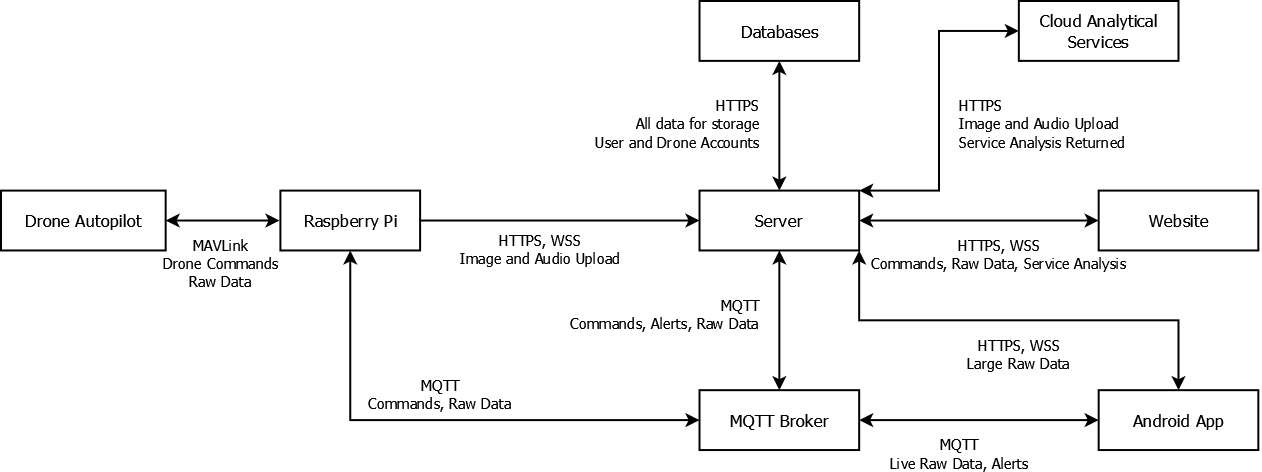
\includegraphics[width=1.5\textwidth]{System}
\end{figure}
\end{landscape}

\section{Background}
\subsection{Motivation}
Whilst there is a growing trend for drone usage in search and rescue operations, this often requires a trained manual operator. With the increasing accuracy and improvements in machine learning techniques, both local and remote AI control of drones is becoming a reality. However, machine learning algorithms often require extensive computational power, and are not suited to be executed locally on a drone. Additionally, any behaviour learned is lost should a drone be destroyed. Off board, on-ground processing is a solution to this. 

The use of drones in search and rescue is not only a very active field of research, there are also an increasing number of successful use cases \cite{UAVUseCase}. \emph{Search} can be considered the more important part of search and rescue, as without a person's location known, they cannot be rescued. Small-scale drones tend to be the most common design of Unmanned Aerial Vehicles (UAVs), as they are most suited to helping \emph{search}; from their unique viewpoint, they can gain greater visual information in a much shorter time, especially if more than one drone work in collaboration \cite{UAV}. However, these drones still require a skilled operator, which may either be unachievable or a poor use of limited resources.

During a \emph{search} operation, time is of the essence. There are two main ways to reduce this time. The first is simply to speed up the process, while the second is to parallelise the task. In most search and rescue situations, the task cannot be sped up, but is parallelised by increasing the number of people. The use of UAVs is one of the few ways to speed up the search processes, by virtue of being able to cover the same ground more quickly. Parallelism is achieved in a similar manner, by increasing the number of UAVs in use. Any reduction of the search time is of great help to rescuers. 

\subsection{Previous and Alternative Research}
Although research is being conducted into making drones fully autonomous, as is pointed out by Tomic et al  \cite{Autonomous} UAVs can only support a lightweight payload, which greatly restricts the computing power available. This is especially important for autonomous drones as they rely heavily on machine learning algorithms for functionality such as speech recognition and visual recognition. These are typically dependent on computationally intensive neural networks \cite{Neural}, which currently cannot be deployed on the microprocessors light enough to be used as a UAV payload. Whilst there exist a range of libraries supporting image and speech recognition on mobile devices, these are not suitable for this application due to two major issues; the computational complexity required for higher accuracy, and power consumption. 

`Offline' techniques do not tend to use neural networks, and are even less likely to use deep neural networks. This is because they require a large amount of mathematical computation when training and using the network; deep neural networks are notoriously hard to optimise \cite{DeepAI}. In theory they can be implemented on small devices such as a Raspberry Pi, and indeed sometimes are \cite{DeepPi}, but even with the Pi's processor running at maximum image classification can take ~20 seconds. This is much too slow for real-time search and rescue. 

In addition, power consumption must be considered. In all examples such as the one cited above, the microprocessor has a stable mains power supply. On a drone, there is no such source. The maximum current the Pi can draw is 1A. Given that the Pi takes 300mA when idle, the PiCam module takes another 250mA, a communication module with the ground will require a further 200mA, and peripheral sensors will require another 100mA or so, there is very little room to power the CPU or GPU to implement onboard processing. Whilst computation could be expanded by adding more processors, as is done by Tomic et al \cite{Autonomous}, there comes a point where, given that the lifting capability of the drone is fixed, moving computation off board is the only option.

\subsection{Potential Solutions}\label{PotentialSolutions}
Off-board processing does not necessarily need to be remote. AI can be implemented on the ground, but locally with a mobile unit. Although currently only implemented with small devices such as a laptop, a much larger and more powerful amount of computation could be provided for instance from a van containing a small computing cluster. Whilst a laptop is greatly mobile and easily obtainable, the advantages it provides over on-board processing are relatively minor. A small computing cluster would provide computing power multiple orders of magnitude larger than on-board, and still have a very low latency. However, the major drawback of this is a very large initial cost. In an ideal world this may be the perfect solution, and a viable option for a well-funded governmental rescue operation.

An alternative solution to this problem, which is growing ever more popular, is the use of the `cloud' to carry out large data storage and computationally expensive tasks \cite{CloudRobotics}. Although not new in concept, given the increase in availability of commercial cloud service providers in recent years the idea of a remote AI is becoming more of a reality. Analysis of cloud computing systems has shown them to have performed well in many desirable areas, such as scalability, portability, and maintainability \cite{SoftwareArchitecture}, which are traits that are becoming more important in the digital age and to this project. 

Given that the drone already has a communication link with the ground for control, this requires little expansion in terms of the hardware or power consumption of the drone; the communication module will draw more current as it transmits more frequently, but the device will still consume less power than if it were to implement local computation as described above. An added benefit of cloud services, or conversely a restriction of onboard or local processing, is the ability to use proprietary services, such as the Tone Analysis described later in this report.


\section{Requirements Capture}
This project is intended as a proof-of-concept, rather than a solution that can be implemented instantly, and therefore the requirements capture can be done through a combination of the developers intuition and discussion with the client, IBM. Additionally, as the work is not being based off any prior implementation or research, and there was little to no experience with the majority of the concepts involved in this project, a large amount of change is expected throughout the project as to how it is actually implemented. This should not, however, greatly affect the overall aims.

The Requirements Capture and Specification of this system were initially vague, and intentionally so. This was to allow a high level of flexibility and independence for the developer to proceed as they wish, whilst achieving larger-scale aims. This was also a reflection on the lack of prior experience with aspects of the projects, such as drones, web development, cloud services and asynchronous programming. The flexibility therefore facilitates development with a very steep learning curve.

As this was an industrial project, the Requirements Capture and Specification mainly came from the client, IBM. Initially they were neatly split into three parts.

\begin{enumerate}
\item A deliverable of a drone must be made. This should be remote controlled, with a mind to it being autonomous in the future. It should act as a data capturer, with a microphone and camera attached.
\item A deliverable of a server must be made. This should incorporate connections to a variety of suitable IBM services, and use data from the drone and analysis from the services to send intelligent commands back to the drone.
\item The resultant information and analysis from the system should be fed back to a user. 
\end{enumerate}

These very simplistic requirements were expanded and refined in the first few months of the project, leading to the Project Specification that was included in the Interim Report. This has been included here, with refinements and updates. The majority of the specification below was met, and any deviations are explained in the relevant Implementation or Testing section. For the focusing of aims and evaluation, a use-case of `search and rescue` was used throughout the project. The project should also bear in mind the intention for future development regarding autonomous control and command of the drone. Although this is beyond this project's scope, thought should be given towards architectural decisions to aid this future plan. 

Although autonomous drone control featured in the Interim Report, reviewing the original client specification and discussion with client has confirmed that the Interim Report was inaccurate in terms of its specification and requirements. The autonomous control is no longer a core part of the project, whereas the user feedback became more important. This had led to some unevenness in the time spent and hence quality of each section. The drone control is well established for a project expansion, whereas the user feedback is perhaps not as robust as ideally it should be. 

\subsection{Project Specification and Deliverables}
\subsubsection{Drone}
The `drone' is a self-contained unit consisting of a quadcopter drone frame, being assembled by the developer, with an autopilot device attached. This autopilot can be controlled either via remote control, as is typical of drones, and/or via direct connection through a set of telemetry IO pins. In this system, these IO pins will be connected to a Raspberry Pi's GPIO pins, and the Pi is to be carried as a drone payload. The Pi can therefore send signals to the drone autopilot in a similar manner to a remote control, for instance increasing the throttle.

The Raspberry Pi will be connected to the internet, initially via a WiFi connection, however this may be changed to a 3G link depending on the requirements of the connection and the level of data transfer. This link provides access to Bluemix, through the HTTP and MQTT protocols. The HTTP connection provides a large data upload link to Bluemix, for example images and audio recordings. This connection is made on a file-by-file basis. The MQTT protocol is different; as it is based on a publisher/subscriber model, it requires a `stay alive' connection to be established initially. Its purpose is to allow movement commands to be pushed to the Pi from Bluemix. Small-size status data will be sent from the Pi to Bluemix, such as GPS coordinates and sensor readings, via the MQTT protocol.

The Pi will be capable of a variety of data collection methods, however the primary one will be `vision', in the form of a Raspberry PiCam. This is a small, very compact camera connected via a dedicated ribbon cable to the Pi board. It is capable of still images with a resolution of 2592x1944, or video at 1920x1080. In this project I will be using still images, as this allows use of image recognition services which currently don't support video. The secondary data collection method will be audio, collected via an external microphone. Other planned data sources also include temperature and drone location, with both GPS coordinates and altitude.

\subsubsection{Server}
For reasons explained in further detail within the Analysis and Design section, the IBM Bluemix platform was chosen to be the primary provider of the cloud services. The `server' deliverable will consist of an application which is run in the cloud on a remote server. As stated, this will be run on Bluemix with the application having its own designated domain, currently http://drone-nodes.eu-gb.mybluemix.net/, through which the HTTP REST requests will occur. The server will receive the data uploaded from the drone, and will store it, process it, and return feedback to both the drone and Android via the MQTT protocol. The central component running on the server will be written in NodeJS. The `intelligence', which decides how to reacts to the analysis the services provide, will be written as a NodeJS component running on the server.

Bluemix services, all provided by IBM, that are expected to be used in the deliverable include:
\begin{itemize}
    \item Cloudant Database. This is a noSQL database built on top of CouchDB. This will be used to store all data, whether raw images from the camera or the results of analysis.
    \item Internet Of Things Foundation. This is a wrapper around an MQTT broker, providing the publisher/subscriber control.
    \item Visual Recognition. Service that takes as input uploaded images and returns a set of labels with associated probability values, which aim to describe what the image depicts.
    \item Speech To Text. A service based on a neural network that analyses input audio and returns transcripts of intelligible speech.
    \item NodeRED. This service provides a graphical interface for Node.js, with each `node` on a flowchart representing a Node.js module. Although it allows rapid development, it was decided early on in the project that due to its lack of customisability it was not used. 
\end{itemize}


\subsubsection{Feedback}\label{Feedback}
Drones in a search and rescue operation are inherently mobile, as are any operators. A method of passing data back to a user should therefore reflect this. Not only this, but the feedback should be user friendly, ruling out the simplest option of forwarding the server log files.

An Android application was chosen as the primary feedback method. Android devices are usually small and highly-mobile, with a low hardware cost. An app can be easily integrated with the server component via the ubiquitous support of HTTP, and by adapting an existing IBM Android application to support MQTT communication\cite{iotStarterAndroid}. The app should be able to present to the user live information about the current status of the drone(s), and the result of any analysis that the server may do. The information that the app could show includes, but is not limited to: drone location and status; direct images, audio, and sensor readings; direct feedback from the cloud services such as image labels; and filtered or interpreted analysis.

\subsection{Assessment Metrics}
As this is a proof-of-concept system, the primary concern and method of evaluation is that the system functions as desired. A set of scenarios and system responses were defined as a measure of desired system behaviour(see Appendix \ref{scenarios}). Although due to the change in the system requirements described in the top of this section a greater focus has been placed upon the user feedback, these scenarios are nevertheless still indicative of desired system behaviour, and are therefore one of the primary methods of evaluation. Fortunately, this shift in requirements did not require too great a change in the implementation, and has led to the system meeting a wider range of specifications.

However, this system does have a potential real-world application, and the performance of the system should be investigated to ensure it is viable. The main characteristic of this system's performance is the latency between the drone emitting stimulus, and the server emitting a response dependent on the feedback from the services. The overall feedback from the services can be investigated, but is not an aspect of the system which can be controlled. However, the feedback may be affected by the quality and density of the input data, which is adjustable. Therefore the effect that this different quality data has on both the system latency and the system response will be inspected. System latency should be minimised, whilst maintaining reasonable system accuracy.


\section{Analysis and Design}\label{AnalysisAndDesign}
This project was tackled with an AGILE methodology\cite{agileManifest}. This means, as the name would suggest, being flexible and adaptable to change. Throughout the project, the focus was on creating a working solution, rather than purely attempting to achieve an end goal. This fits in perfectly with a proof-of-concept project. First, develop just one pillar of the concept, and make sure it works. Add more, ensuring functionality at each stage, until the whole is complete. One of the primary principles of the Agile Manifesto is ``Working software is the primary measure of success``\cite{agileManifest}, hence the focus on small and constant evolvement. Due to a modular approach, any change in requirements or resources can be more easily adapted to. 

The project specification quite succinctly identifies the necessary components and deliverables, as the specifications are by nature component definitions as opposed to system characteristics. What does require more thought is how each component is built and designed. The majority of component-specific design choices are described in the relevant Implementation sections; due to the agile mentality the design often changed, usually in an forward evolving manner. This was especially prevalent in the Server component, due to lack of experience in NodeJS and practical networking practices. However, a few overarching themes are discussed below.

\subsection{Architectural Choices}
Modularity and separation are traits that encouraged in many aspects of software engineering, and are focussed on in this project. If a component has many tasks to do simultaneously, these are separated and implemented concurrently rather than sequentially. A monolithic approach tends to be more archaic, and have often been replaced with a microservices approach. Examples of this are multi-threading on the Raspberry Pi, and the asynchronous nature of NodeJS.

\subsection{Cloud Services}
An example of the microservices architecture is the use of individual and independent cloud services, rather than implementing all functionality in a single `black box`. Should one fail, the others should be unaffected, and the system should be able to handle with this in a pre-determined manner. 
\subsubsection{Providers}
There exist a number of Platform as a Service (PaaS) providers, but three of the most popular are summarised below.
\begin{itemize}
    \item Microsoft Azure - well-established provider, high cost with no free-tier
    \item Google App Engine - offers a free-usage tier, but has more limited machine learning services
    \item IBM Bluemix - more recently released, offers unique `Watson' intelligence.
\end{itemize}
As this project was a collaboration with IBM, Bluemix was the provider chosen. However, there is good reason for this, primarily due to the unique services and functionality which Bluemix provides related to machine learning and data analytics. These have been developed following IBM's success with the intelligent machine Watson, and are likewise named Watson Services \cite{Watson}. The insights provided by these unique services have been experienced in previous work with Bluemix \cite{EdgeOfSpace}, and verified by recent research to test Bluemix's capabilities \cite{Sentiment}. Especially relevant services that Bluemix provides, which are not available from alternative PaaS providers, are the Visual Recognition and Tone Analysis services.

\subsection{Security and Safety}
Security is an essential aspect of any modern system. This project, despite only being a proof-of-concept application, requires a reasonable level of software security. Potential risks from a lack of security include:
\begin{itemize}
	\item Loss of data, both drone collected and personal data
	\item Abuse of cloud services - `free-tier` usage of cloud services all have a usage limit. If exceeded, payment is required
	\item Physical damage or theft of drones, as flight commands can be sent from server
\end{itemize}
The focus for the mitigation of these risks is the central server, and the communication it has with peripheral components. Sufficient steps will be taken throughout the development process to ensure that any security risk is minimal.

There are practical safety concerns when regarding aerial vehicles. Well before any flight takes place, the appropriate regulations from the Civil Aviation Authority will be read and understood.

\subsection{Documentation}
Any software system is only as good as its documentation. If future users or developers cannot understand and maintain a codebase, it has little purpose. Therefore this project will strive to provide concise and clear documentation of all aspects, through a combination of code commenting, API documentation, and JavaDoc documentation. The work of this project, following its completion, is going to be passed to and continued by developers at IBM. This only reinforces the requirement for effective documentation.

Git will be used as a Version Control System (VCS), with repositories hosted remotely both on GitHub.com and IBM's repository hosting website Jazz\cite{jazz}. Not only will this ensure a reliable backup for the codebase, but git repositories stores data about development throughout the lifetime of a project. As well as static documentation, historical development information can be useful in understanding a code base, for understanding architectural and software decisions\cite{crimeScene}. Following the project's completion, these repositories will be made public and passed to IBM.

A user guide at the end of the report details fully instructions for use and documentation details.

\subsection{Synchronisation}
This is a time dependent system, as collected data has a useful `lifespan`. There is little point in reacting to hour old images. Therefore, the time that specific items of data is captured must be recorded and stored alongside the data itself. This becomes slightly more complex when the data is used across many different systems and software languages. The format of the timestamp must be supported and understood by each system. To facilitate this, all timestamps and measurements will be done in milliseconds since epoch, a (currently) 13 digit number that represents the time passed since 1 January, 1970. It must be ensured that all systems have the same current time value.

As well as time synchronisation, consideration was given to standards conformance, both externally and internally defined. For example, across the languages used of Python, NodeJS, JavaScript, and Android, where possible the use of Java-style `camelCasing` is used uniformly.

\section{Implementation}
This section explains in details each of the 3 primary deliverables. Although a large amount of change occurred throughout development, it is only the final solution which is presented here, to ensure a clear overview. As this project is a \textit{design and make} project, as well as being an evolving proof-of-concept, this section can be regarded as one of the most important of the report. Many of the decisions regarding the final implementation are described and justified within, as well as discussions on earlier designs and their flaws. 

To give a sense of the complexity and interaction between the components, Figure \ref{fig:CommSingleUpload} shows the communication and data flow for the upload of a single image. The file, with corresponding GPS data, is uploaded to the server, and subsequently the database and image recognition services. An alert is sent to the website via a websocket, and to the Android app via MQTT, to trigger these components to load the latest image. The image recognition returns a set of labels, which are again sent to the website and Android app via different channels. The labels are analysed, and a subsequent command is sent back to the drone via MQTT.

\begin{figure}[h]
\centering
\caption{Communication and Data Flow For A Single Image Upload\label{fig:CommSingleUpload}}
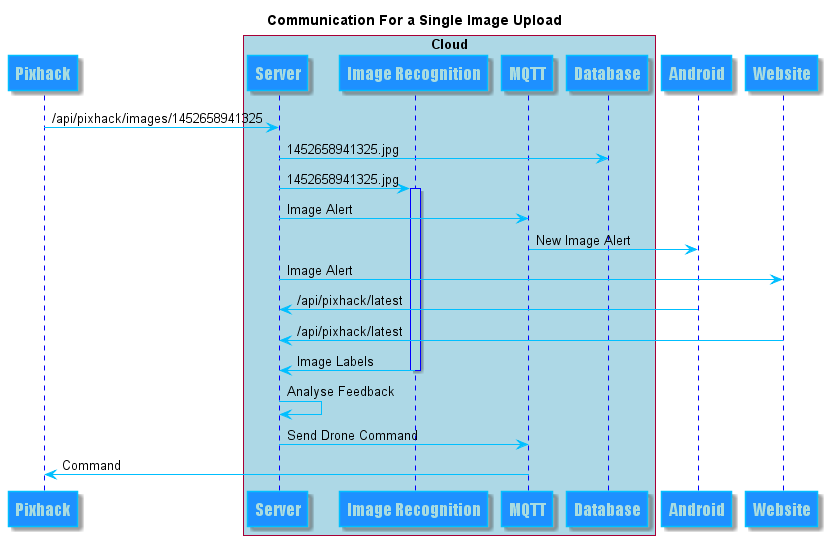
\includegraphics[width=\textwidth]{CommSingleUpload}
\end{figure}
 
 Everything described in the Implementation Section has been implemented and is part of the working solution. 
 
\subsection{Pi and Drone}
The `drone` deliverable consists of two major components, a Pixhack autopilot and a Pi microcomputer. The autopilot is responsible for the usual actions of a drone, including: receiving remote control signal, and converting them into calibrated motor outputs; using internal sensors, such as attitude, altitude, and GPS position; autonomous flight following a series of pre-defined waypoints, using the sensor readings. It operates using firmware written in C, and is not capable of advanced computation or communication. The Pi is a microcomputer running a Linux distribution. It is highly versatile and customisable, and supports higher-level languages such as Python. 

In this system, the drone frame carries both the autopilot to control flight, and the Pi to allow the more advanced functionality. The Pi and Pixhack are connected via a serial port, and communicate using the MAVLink protocol. The Pi is responsible to collecting all desired data for the system, including images and audio from Pi peripherals, and altitude and GPS information from the drone. The Pi constantly transmits this data to the server, and will act upon any commands it receives from the server.

Figure \ref{fig:DroneDiagram} shows a simplified diagram of the Drone deliverable hardware. Circles are the component inputs and outputs, while diamonds are communication devices. RC is the Remote Control receiver, and ESC is the Electronic Speed Control, which converts the signal from the autopilot into a 3 phase signal for a motor. The firmware on the Pixhack is open-source and unchanged, whilst the software development for the Pi is described below.

\begin{figure}[h]
\centering
\caption{Diagram of `Drone` Deliverable\label{fig:DroneDiagram}}
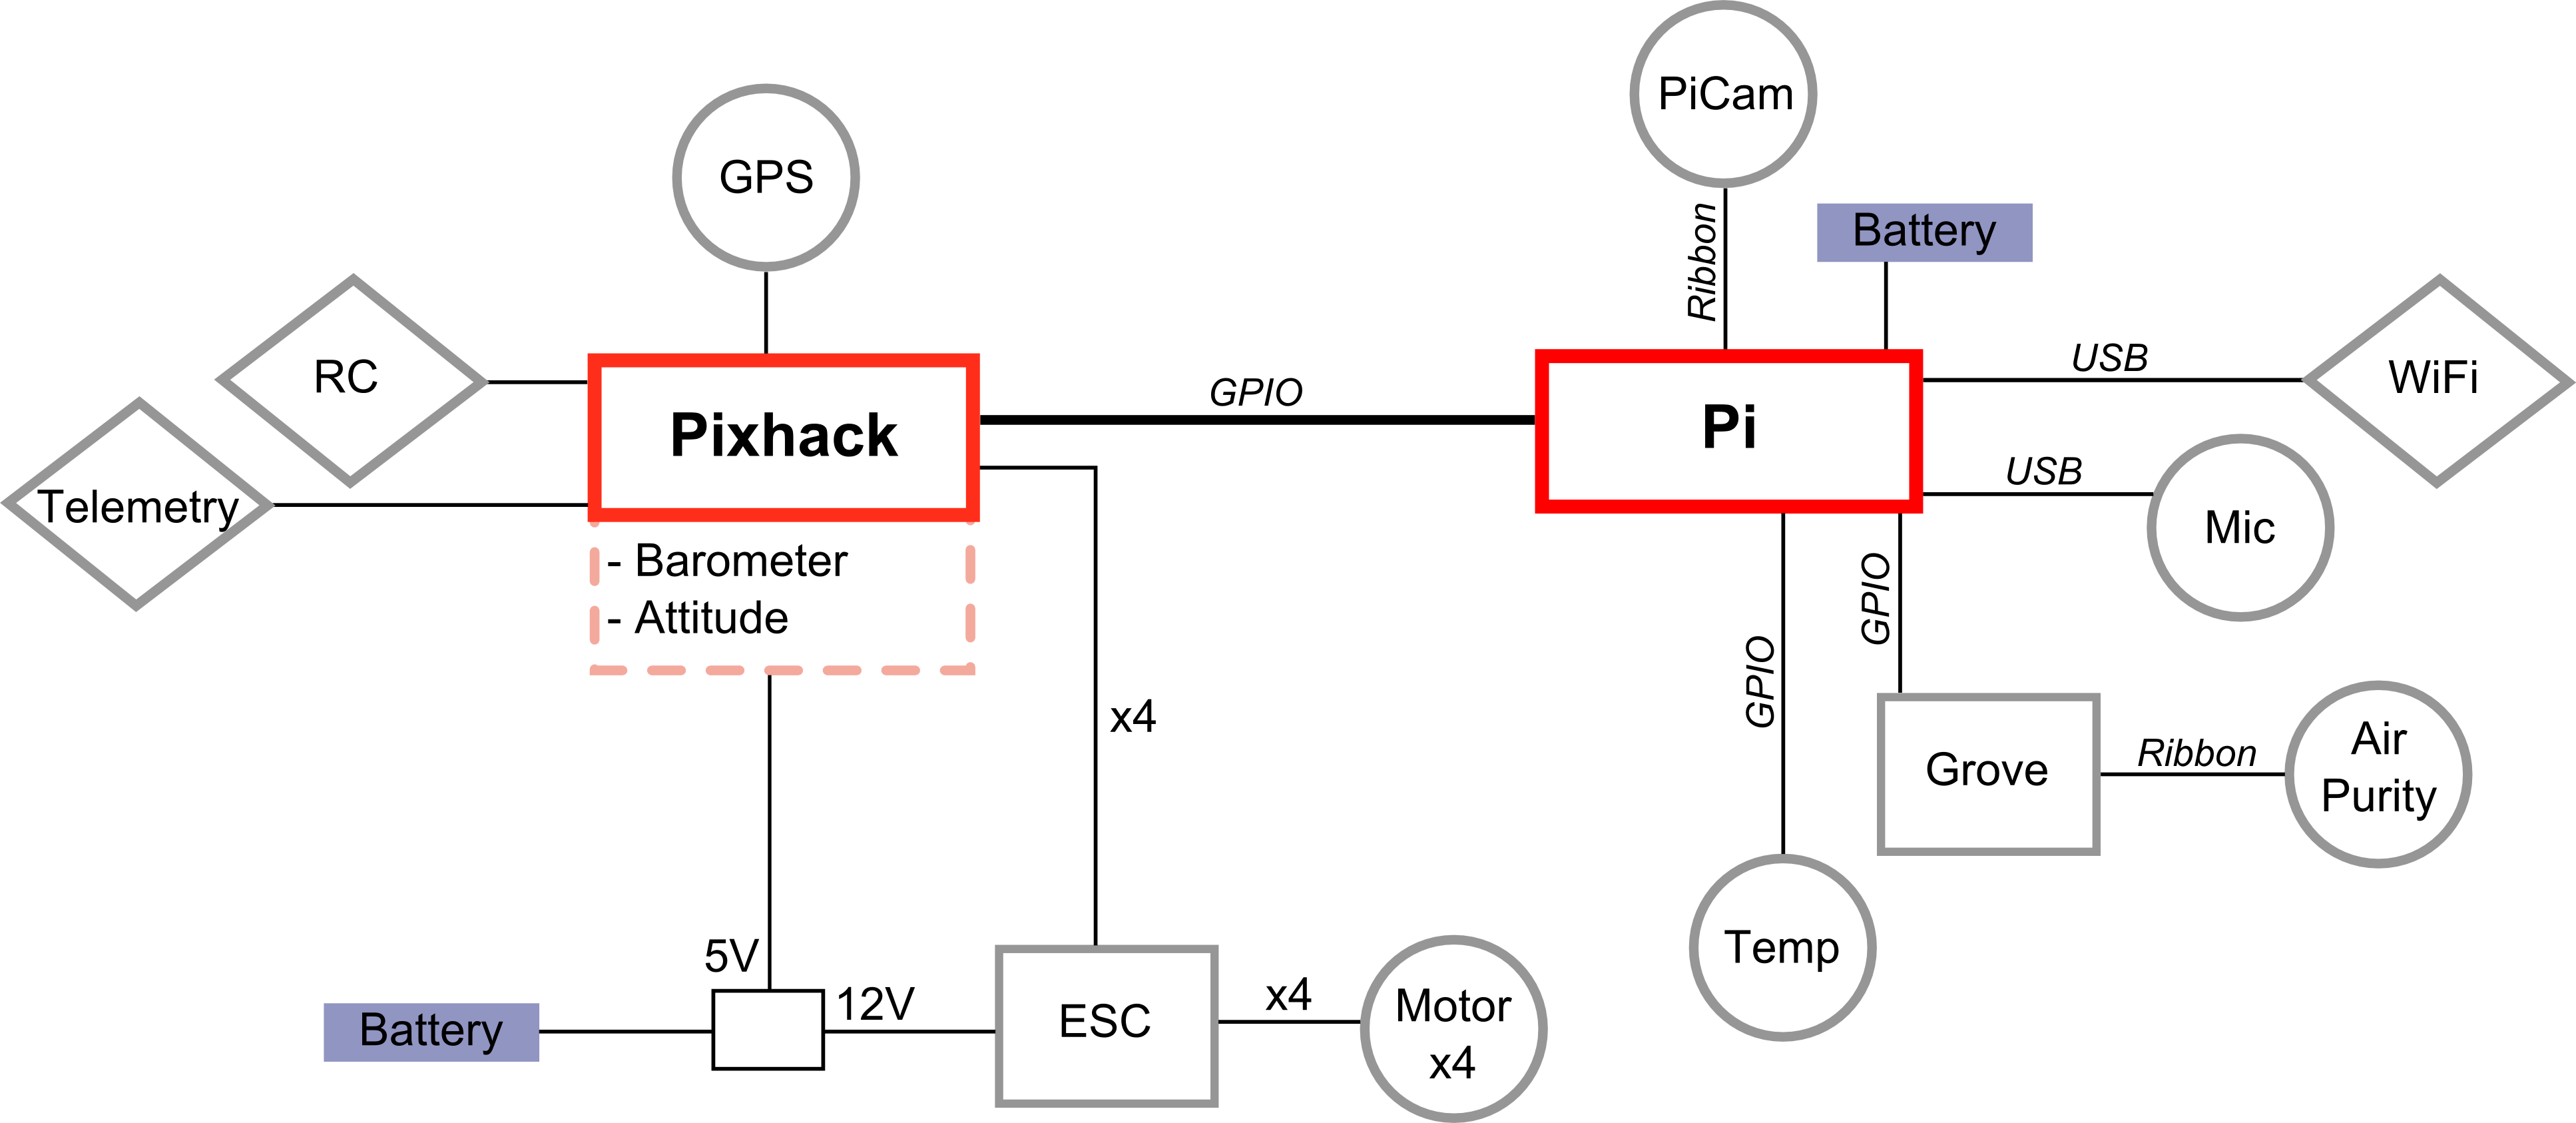
\includegraphics[width=\textwidth]{DroneDiagram}
\end{figure}


//TODO Attach photos in appendix

\subsubsection{Physical Assembly}
The Raspberry Pi was bought through Imperial College EEE Stores, including peripherals such as a WiFi module, PiCam and microphone, and Grove Pi shield. The drone itself arrived mostly in a bulk delivery, the order having been placed by IBM. 

Following a long delay in the arrival of the drone components, it was assembled in March. The assembly itself presented no major problems, with the majority of components being modular plug-and-play units. Throughout assembly and further development, equipment was bought or replaced with some regularity. Some was planned, such as the RC devices, whilst replacements were unexpected delays. The battery of the drone arrived later than all other components, and then later had to be replaced. The battery needed a specific Lithium Polymer (LiPo) charger, and required additional connectors to attach to the drone power board, and a remote control transmitter and receiver were sourced. Although `Grove Pi` sensors were provided in the initial bulk delivery, the Pi shield required to use them was not. Whilst this list is not comprehensive, it gives a sense of the many requirements of a hardware system. The delays for these components, other than those mentioned in section \ref{MajorDelays}, were individually minimal in their effect upon the project, but were frequent. 

\subsubsection{MAVLink}
MAVLink is a lightweight communication protocol, which packs small C-structs over serial data channels\cite{qGroundMavlink}. It is a non-commercial open-source project, which is used as the primary method of communication in many modern unmanned aerial vehicles. The Pixhack autopilot uses this protocol to communicate with both ground stations and the Raspberry Pi. Both status and sensor data is transmitted, as well as the ability to send commands and instructions to the vehicle. Wrappers around the MavLink protocol are provided in Python by pymavlink, a library in the MAVLink git repository.

\paragraph{Ground Stations}
`Ground Stations` are software applications that interact with aerial vehicles for preflight calibration and flight control. Given the recency and open-source nature of the MavLink, there are many ground control stations, yet they are all likewise non-commercial ventures. Regrettably, this can mean they are often unreliable, especially when things go wrong. As described in \ref{MajorDelays} the first Pixhack board used was faulty. The ground stations would usually give vague and unhelpful feedback upon the failure of an operation, meaning identifying problems was difficult. The primary ground station used in this project was QGroundControl\cite{qGroundControl}, as not only was it the recommended application for Pixhacks, but it also provided a useful MavLink package inspector. 

\subsubsection{Pi Development}
The software on the Pi is written in Python, due to the rapid speed of scripting and the large amount of support available. The tasks that the drone has to undertake involve large amounts of blocking and low CPU usage, such as a file upload, or sensor reading. Therefore, the use of threading is extensive. The threads are summarised below, with each starting at program boot and entering an endless loop. 
\begin{itemize}
	\item The main, primary thread. After initialising variables and spinning off threads, this regularly checks the \texttt{PiCommandQueue}, and will act upon any commands it receives such as changing the mqtt upload interval.
	\item \texttt{sensorThread} reads Pi attached sensors, such as temperature and airpurity, editing the \texttt{sensors} object.
	\item \texttt{droneThread} communicates with the drone autopilot. This is a rather heavier thread. After establishing a connection with the drone, this threads repeatedly attempts to receive a message from the drone, and then checks to see if any commands are on the \texttt{MavCommandQueue}. Incoming messages are passed through a switch statement, and may update the \texttt{sensors} or \texttt{gps} objects. Commands are looked up in a dictionary from the provided string, and the corresponding function is carried out with the provided arguments. 
	\item \texttt{imageThread} regularly captures images using the PiCam, using settings from the \texttt{status} object.
	\item \texttt{audioThread} captures audio from the microphone in two methods. Either audio is captured and directly streamed to the server, or audio files can be captured based on volume detection. These files may be converted to mp3, or saved as uncompressed WAV.
	\item \texttt{imageUploadThread} continually finds the latest file in the image folder, and uploads this to the server. A check is made to ensure the image has not already been sent.
	\item \texttt{audioUploadThread} does the same as the \texttt{imageUploadThread}, but can be put on hold if the Pi is streaming audio.
	\item \texttt{mqttThread} connects to the MQTT broker. It regularly sends the \texttt{sensors} object, and will handle any commands sent from the server, adding them to the \texttt{PiCommandQueue} or \texttt{MavCommandQueue}
\end{itemize}

Due to the many threads operating on the same objects, thread-safe programming must be used. The message queue are instantiated as a thread-safe FIFO queue, and threading locks are used for access to the \texttt{sensors}, \texttt{gps} and \texttt{status} objects.

The majority of development of the python on the Pi progressed as planned, without any major problems or architectural changes encountered. It was clear from early on that threads should be used due to the many blocking tasks, and although issues were encountered with adding security to satisfy the server requirements, and with ensuring objects were thread safe, these were not unexpected or exceptional. However, there were significant issues with the droneThread, as described in \ref{MajorDelays}.

\subsubsection{Major Delays} \label{MajorDelays}
For a period of around 6 weeks, there was serious difficulties in getting the autopilot to behave as expected. A large amount of time was spent during this period trying to debug and understand the issue, but eventually it turned out to be faulty hardware. 

The issue was that although the autopilot would communicate as expected with MavLink, there were notable omissions from the packets received, such as RC value, and output servo values. The drone would not `arm`, the state needed to begin flying. Due to inexperience with the protocol and aerial vehicles, and a complete lack of any form of error message, it was assumed that is was a configuration or software error. Large amounts of time was spent trawling through online web forums and literature. Note that due to the non-commercial nature of MavLink and related components, there was no official support other than the company the drone was purchased from. 

Many different approaches and solutions were attempted, and certain issues were fixed; a junction on the provided Pulse-Position-Modulation (PPM) encoder required soldering to provide power to the RC, an issue which was only known about due to contacting technical support from unmannedTech\cite{ppmSolder}. The lack of provided documentation meant there were a number of similar issues throughout the project. However, none of these fixed the primary issues. Eventually it was found that the SD card of the autopilot, once it had been reformatted due to it being corrupted, showed an error message `PX4IO board not found`. This lead to attempts to fix the firmware on the autopilot, which forums indicated was the root of the issue. However, this, combined with the inability to power the Pixhack directly (only indirectly via the Electronic Speed Control module), lead the technical support at unmannedTech to suspect a hardware fault, and to return the board\cite{px4ioNotFound}. 

The board was indeed faulty, and after receiving a replacement the board behaved as expected, and is able to arm correctly. However, due to this extensive delay, development regarding the control of the drone was severely restricted. Autonomous control was not fully achieved.

One advantage of this issue was that due to line-by-line debugging of the large pymavlink library, a solid understanding of how it is implemented was gained. It also allowed time for greater development of the central server component of the system.

Another substantial delay was trying to install \texttt{ffmpeg} on the Raspberry Pi (see \ref{AudioFile}). \texttt{ffmpeg} has been removed from the official repositories, and attempting to build from source did not work. Different sources and configuration were attempted, with each source build taking 6 hours on the Pi. Although a prebuilt binary was eventually found, this did not work due to errors with previous configurations. Eventually, the operating system was reinstalled, upon which the prebuilt binary worked as expected. This also allowed an exact list of installation requirements on the Pi to be generated for future use - see \ref{UserGuide}. 

\subsubsection{Audio File Conversion}\label{AudioFile}
Initially, audio was only captured by volume activation, and saved as an uncompressed WAV file. This is due to the requirement of the Speech to Text service requiring input files of a specific format. However, uncompressed WAV files are very large, and therefore take a considerable time to upload. This means any analysis returned from the service is likely to be too old to be useful. Therefore, data compression was implemented. mp3 is a standard, high-compression audio format. The tool \texttt{ffmpeg} was used for this conversion, due to a lack of a suitable Python library to execute the conversion. After the data is captured, it is passed to the \texttt{ffmpeg} tool as a command-line process, which saves an mp3 file format. Once this file is uploaded to the server, an npm (see \ref{npm}) module\cite{npmlame} providing access to \texttt{lame} was used to decompress the mp3 into a WAV file, which can be sent to the Speech To Text service for analysis. 

\subsubsection{Streaming}\label{Streaming}
Once the drone rotors were attached and the drone could run, it became clear that noise activation would not work as a method to start and stop audio capture. The volume of the drone rotors was far louder than expected, and would drown out any voice. The alternative is to have constant recording, with a set time interval to create discrete files. However, not only does this raise the issue of sentences being split over files, but the Speech To Text service cannot cope well with high levels of noise, as shown in \ref{Testing}. 

The human ear, however, is well known to be very adapt at the cocktail party effect\cite{cocktailParty}. A human may be able to make use of audio that the intelligent services cannot. Therefore, the functionality of audio streaming was added to all components of the system. If the appropriate option is enabled on the Pi, file capture stops, a connection is made to a websocket on the server, and all audio data is directly uploaded as binary data. The server receives this data on one `uploaded` websocket, and broadcasts it to any listeners on the corresponding `listen` websocket. The Android app can choose to stream audio, in which case it connects to the `listen` websocket, and plays any data received.

\subsection{Node JS Server}
The system requirements specified that a central server must exist, both to coordinate communication between all remote components and to analyse and act upon this communication. This will require many asynchronous actions occurring at the same time, which will have different requirements. Connections to IBM services may have a very high latency due to the time required to implement the analysis, yet require little server processing. Assessing and acting upon the results from IBM services will require server processing, yet no external connections. IBM Bluemix provides a server container, but the server implementation must be written in a language of the developer's choice. 

NodeJS was chosen as the language for the server. This was for the two main reasons of existing support for IBM services, and its suitability for this project's requirements. Although the IBM services do all provide a HTTP API, there exist a NodeJS SDK, which creates objects to include and interact with rather than interacting directly with the API\cite{githubWatsonCloud}\cite{githubCloudant}\cite{githubDB2}. This would save a vast amount of time and effort throughout the project. Secondly, NodeJS is suitable for servers which are event driven, with non-blocking asynchronous actions\cite{smackdownPHPNodejs}, which is the style of this project.

NodeJS has only a single primary thread of execution. To enable handling of multiple tasks simultaneously, it uses the technique of callbacks rather than blocking. This means that a `callback` is passed as an extra argument to a function call, and this is executed when the function call returns. This can get confusing as the callback is often declared inline. A typical function call is below:

\begin{lstlisting}
databaseObject.someFunction(arg1, arg2, function(error, result){
	if(error){
		// Handle Error. Usually requires a return, or else handle result
	}
	// Handle Result
});

\end{lstlisting}  

In the body of someFunction, there will be some action that can be conducted in the background, such as a file interaction or networking. This can be handled without interaction from the primary thread, until more work such as executing the callback is required. Although somewhat different to conventional programming and tricky to understand initially, this method of handling asynchronous actions results in a powerful tool that is capable of doing many actions simultaneously. 

All of the IBM services used, each of which are described in more details below, are interacted with via NodeJS modules as stated above. At server boot, a credentials JSON object, VCAP\_SERVICES, is read. In Bluemix, these are set as environment variables, where as locally the credentials are read directly from a file. The credentials are then used to instantiate the object, and for some a connection is made immediately.

Figure \ref{fig:ServerDiagram} shows a class diagram of the NodeJS codebase, giving brief descriptions of each module's function; each module is defined in its own file, and included by using the NodeJS directive `require`. This highlight the modular nature of development; initially the majority of the functionality was included in the main `app.js` file, before being expanded. 

\begin{landscape}
\begin{figure}
\centering
\caption{Class Diagram of NodeJS Codebase\label{fig:ServerDiagram}}
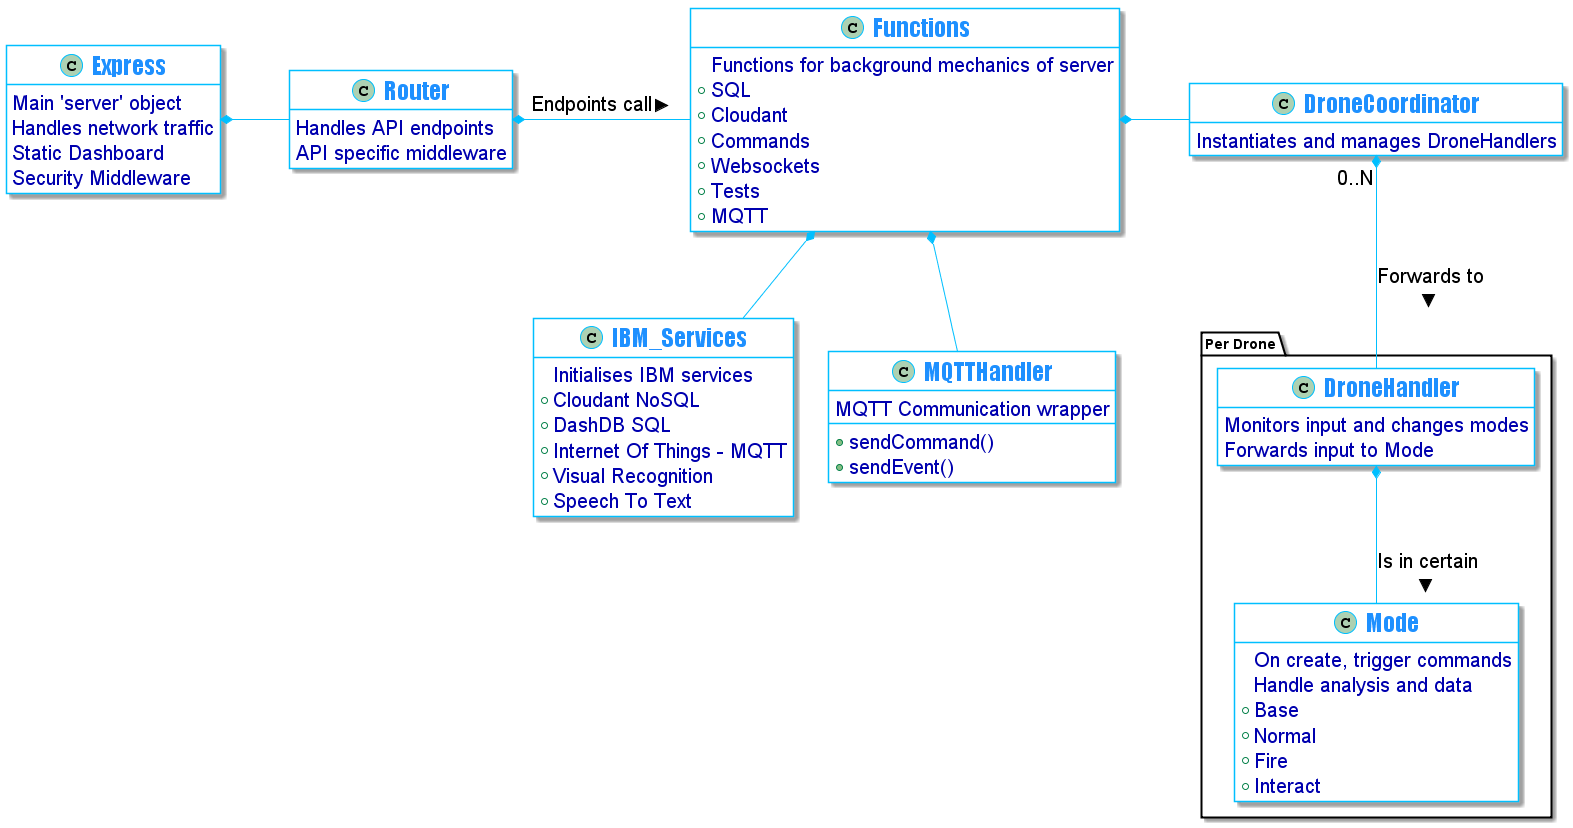
\includegraphics[width=1.5\textheight]{ServerDiagram}
\end{figure}
\end{landscape}

\paragraph{npm}\label{npm}
One of the very useful features of NodeJS is its package manager, npm. As well as the basic functionality of being able to install and update packages manually, npm uses the file `package.json` to manage dependencies, implement version control, and coordinate installation and start scripts for node amongst other things. This greatly simplifies project setup and maintenance. The instruction `npm install`, executed in the project's root directly, will install the specified versions of all dependency modules into the directory node\_modules, including those required for testing and development, and run the script `install.sh` which generates the projects documentation.   

\subsubsection{MQTT Service}
At boot, the server registers itself as an Application on the MQTT broker, subscribing to all device events, and therefore picking up any messages from the drone. This service is used in the server to collect drone messages, send drone commands, and also send messages to other connected clients such as the Android app.

Later in this project, when MQTT was not available or for less suitable data content such as audio streaming, websockets are used in a very similar manner. However, MQTT provides functionality that a simple websocket cannot. MQTT is designed for lightweight communication where network bandwidth is at a premium or intermittent\cite{mqttSpec}. The overhead cost is therefore minimised, and connection from a client to a broker has mechanisms of determining disconnection or temporary loss of contact. As a publisher/subscriber model, MQTT can be connectionless. The server does not need to be online for the drone to emit MQTT packets, and a single emit from the drone can be broadcast to many connected clients. There are three qualities of service (QoS), `at most once`, `at least once`, `exactly once`\cite{mqttSpec}. Given the repetitive nature of drone messages, these are suited to the `at most once`, or default, QoS. Message loss happen, and if is ignored. This removes any need for duplicate handling. However, for more important messages where guaranteed delivery is desired with no duplicates, the `exactly once` QoS service can be used. In this system, commands send to the Drone component use this delivery method.

\subsubsection{Analytical Services}\label{AnalyticalServices}
Two main analytical services are used. Although others were explored, either the input data or response was not detailed enough for use. For instance, the very clear phrase `I need help. I am hurt.` generated no meaningful response from the Tone Analysis service. 
\begin{itemize}
	\item VisualRecognition - used to generate keyword labels off an input image, which originates from the drone. Although the exact details of the service are proprietary knowledge, it is based upon a pre-trained neural network. There is a large set of labels that the service can identify, around 700 unique ones. The service returns any label which has an output score of above 0.5 (out of 1.0). 
	\item Speech To Text - used to generate a transcript from an input audio file, which originates from the drone. The returned transcript also has a confidence score from 0.0 to 1.0. 
\end{itemize}

\subsubsection{Data Storage}
Two methods of data storage are used, a no-SQL database service called Cloudant, and a standard SQL database. Both are managed through a website 'dashboard', and are accessed through a NodeJS module wrapper around a REST API. Both are used as each is better suited for the task for which they are used.
\paragraph{Cloudant}
no-SQL databases can be seen a bit like a 'bin'; any JSON object can be dumped into it, regardless of properties or adherence to a pre-specified specification. This is perfectly suited to sensor data recording, as it means if a new sensor type is added the database requires no alteration, similarly if a sensor reading is omitted. Each record in the database is called a document. It is also possible to attach files, such as JPEGs or WAV files, to a document as an attachment. This is a much easier way of storing large volume data when compared to SQL BLOB(Binary Large OBject). For these reasons, the IBM no-SQL implementation, Cloudant, was chosen as the persistent storage method for all data, other than the accounts described in the SQL section below. 

The Cloudant database was very easy to set up and put data in. However, issues arose when it came to querying data. Due to the fact that the data has no specification, there is no guarantee or knowledge of the data content of the database documents, so it cannot be queried except for with its primary key, '\_id', which is the only enforcement of the database. If not provided \_id is randomly generated, but in this project the use of a timestamp, in milliseconds since epoch, was used as a document \_id for all Cloudant databases. This allowed querying of the data using the id, before indexing was fully established. Indexing is the proper method of querying the database, and requires two steps. First, an index must be made. Next, queries can be run against this index in a similar manner to an SQL query. For instance, an index of the field 'type' is made on the sensorlog databases. This is currently done on database creation. A query can then be run, which uses a selector and the indexed fields to provide relevant results.

\paragraph{SQL} \label{SQL}
The SQL database is provided as an IBM DB2 service, and issued for more static relational data which is text based and doesn't require large file storage. There are two primary tables, `users` and `drones`, the definitions of which can be found in the Appendix (\ref{SQLDefinitions}). Each table's function and column names are fairly self explanatory, with users storing a list of the user accounts, and drones storing registered drones. `salt` and `password` are explained in more detail in the security section, as is the nature of `role`. An SQL implementation is better suited to this nature of data, as it is more rigid and stringent, ensuring mistakes and errors are less likely to occur. Isolation for security is also a good practice. Having a database reserved specifically for security and account information means the system can focus on access more easily, and any damage caused by a weakness elsewhere in the system is minimised. Due to previous experience with SQL, there were few issues with the creation or use of the SQL databases. 

\subsubsection{API} \label{API}
Due to the size limitations of the MQTT protocol, a different method is required to exchange files, such as the audio and images captured by the drone. Not only this, but the MQTT model is not suited for making queries for legacy data, or for static information; as a publisher/subscriber model it ideal for live data. Therefore, the HTTP protocol was used due to its ubiquitous support and obvious suitability. A REST API was created on the server, to facilitate ease of development and to conform to industry standards. 

A RESTful (representational state transfer) API is one that satisfies a range of constraints, including having a client-server model, being stateless, consider caching, and provide a uniform interface. As much as possible, the API in this server attempts to meet these constraints and largely succeeds. It follows a client-server model, is stateless (although the drone control behind the API is not), and provides a uniform interface, for instance by identifying resources individually through the URI. To ease development and due to the relatively low demand on the system, all responses are assumed that they cannot be cached, although in reality many could be. 

An example of an API endpoint is given below. They are often provided in the format of a URI extension, which should be concatenated with the base URI for use. This endpoint would be used to obtain the resource described by the URI, that of an individual image captured by a specific drone.
\begin{lstlisting}
GET    /api/:dronename/image/:docID
\end{lstlisting}
In the API descriptions, `:\textless name\textgreater` indicates a variable parameter in the URI which the server can access\cite{expressDocs}. As mentioned in the sensor development, these are often validated, as can be seen in Table \ref{tab:RequestParams}. If a validation fails, an error HTTP response code is returned to inform the client of an error. A range of HTTP response codes are used within the API, to represent success (200), redirection (302), client error (4xx) and server internal error (500).

\begin{table}[h]
\caption{Request Parameters\label{tab:RequestParams}}
\centering
\renewcommand{\arraystretch}{1.5}
\begin{tabularx}{\textwidth}{>{\centering}p{1.5cm} >{\centering}p{1cm} >{\centering}p{3cm} p{5cm} X}
Parameter & Type & Description & Validation & Failure Action \\ [0.5ex]
\hline
dronename & String & The set of databases to query & Request's cookie is checked to ensure it contains dronename & Return HTTP code 400 \\
timeFrom  & Number & Timestamp in milliseconds since epoch  & Is checked to ensure it will parse to a number & Return HTTP code 400 \\
timeUntil & Number & Timestamp in milliseconds since epoch  & Is checked to ensure it will parse to a number & Return HTTP code 400 \\
type      & String & The type of sensor to data to collect & None & None \\
username  & String & The username to act upon & Ensure the username provided matches that in the cookie, or that the client is an ADMIN & Return HTTP code 401 \\ 
docID 	  & String & Timestamp in milliseconds since epoch & If the docID = "latest", the latest document to be uploaded is returned rather than a client specified docID & None \\ [1ex]
\hline
\end{tabularx}
\label{table:requestParams}
\end{table}

This REST API evolved slowly. In line with the Agile methodology, from the very start the focus was on always to have something working. As an example of the process of development, the process of creating the Sensor endpoints is described below. At each step, it was made sure that the implementation worked correctly before progressing. Some steps, especially later, were part of larger redevelopments but the majority are specific to the Sensor endpoints. The purpose of this is to show the level of thought and constant development that it took to create this functioning API. Note that these are only GET endpoints, and therefore the simplest.

\begin{itemize}
	\item The first endpoint was added directly to the express object with `app.get()`, and `/getSensorData` simply returned a JSON dump of every document in the Cloudant database `sensorlog`
	\item '/getSensorDataLatest' also used the inbuilt function to retrieve all documents, but to order by descending \_id and only return 1, hence returning the most recent document as the \_id is a timestamp. 
	\item Once the Cloudant SDK was fully understood SECTION, querying the database correctly became possible.
	\item The endpoint accepted URI query parameters, for instance `/getSensorData?timeFrom=14235786351`. A selector object was made, and sent to Cloudant as a query. This queried the \_id of the documents. A default value is provided for if no value is specified, allowing the same function and Cloudant query to be used.
	\item The database was indexed for type correctly, meaning the selector could be expanded to include other fields, such as `/getSensorData?timeFrom=14235786351\&type=temperature`
	\item Using the \_id as a field could cause error, as the internal comparison on the database treated the \_id and the selector field as a string. `2` would therefore be considered greater than `14235786351`, as 2\textgreater 1. The field `time` was added to documents and the database re-indexed.
	\item Minimum and maximum values were added to the selector, meaning both a time and value range could be used to select specific documents.
	\item The functionality that an endpoint provided was encapsulated in a separate function, rather than being defined when added to the express object. The function was passed to `app.get()` as a callback function.
	\item Path parameters rather than query parameters were introduced for timeTill, timeFrom, and type. Varying endpoints were created, to support use of a more simple client query. 
	\item Parameter checking was introduced, to ensure that the values of timeFrom and timeTill are indeed numbers, or the key-string `latest`, which would run the query triggered by `/getSensorDataLatest`
	\item An express router was used, meaning the endpoints were added to the router object. This prefixed '/api/' to existing endpoints. 
	\item Security was implemented, ensuring that a user had to be logged in to access these endpoints
	\item The router and related functions were removed from the growing app.js file, and placed in their own files. This required extensive refactoring and testing.
	\item Multidrone support was added, by adding dronename to all paths, and using the dronename to specify which database to query.
\end{itemize}

These steps, and similar steps for all other endpoints, have led to a comprehensive and effective API. A more detailed explanation of the API endpoints can be found in the Appendix (\ref{apdxRestApi}), whilst full user documentation can be found by accessing the public endpoint '/documentation/api', which was generated using apidocs\cite{apidocs}. This contains further details of the API, including how to use it, security restrictions, error messages, and parameter and response definitions.

\subsubsection{Security}
Security is an important issue for any software system, especially for those that are connected to the internet. This can be regardless of whether an attacker gains anything, yet is even more important should that potential be there. Security threats regarding the NodeJS server are detailed in Table \ref{tab:SecurityThreats}, using the STRIDE methodology\cite{stride}.

\begin{table}[h]  
\caption{Security Threats\label{tab:SecurityThreats}}
\centering
\renewcommand{\arraystretch}{1.5}
\begin{tabularx}{\textwidth}{ | >{\centering}p{1.5cm} |  >{\centering}p{3cm} | X  | X |}
\hline
Threat & Description & Practical Method & Prevention \\ [0.5ex]
\hline
Spoofing & Pretending to be somebody else & Edit cookie `user` value & - Make cookie inaccessible to user \\ \hline
Tampering & Modifying without permission & - Access a POST or Delete endpoint \newline - Edit cookie values of username, drones, or role & - Restrict API access to those with session \newline - Make cookie inaccessible to user \\  \hline
Repudiation & Denying to have done something & Edit any data on the server & - Restrict API access to those with session that contains username \newline - Log all API accesses \\ \hline
Information Disclosure & Revealing information without permission & - Access any GET endpoints without login \newline - Access GET endpoint without authorisation & - Restrict API access to those with session \newline - Contain Role within cookie, and restrict access to certain endpoints dependent on role \\ \hline
Denial of Service & Prevent a system from providing service & Overload the server & - Ensure adequate asynchronicity in NodeJS code to handle requests \newline - Rely on Bluemix front server for protection \\ \hline
Elevation of Privilege & Achieve more than what is intended or allowed & - Access any endpoint which doesn't match the Role \newline - Edit cookie containing role & - Restrict access to certain endpoints dependent on role \newline - Contain Role within cookie, and make cookie inaccessible \\ 
\hline
\end{tabularx}
\end{table}
To mitigate these threats, it is clear there is a requirement for a user to have a registered account, with a session cookie for when they log in containing relevant data, that is both tamper proof and should not be used by others. These requirements are satisfied by the use of session cookies and user accounts as described below. Also, to prevent the theft and reuse of a cookie, all transport should be done over SSL, namely HTTPS and WSS. Any request that is not over HTTPS is redirected to the HTTPS version of the URI. Whilst this is not enforced on local development, it is implemented on the Bluemix implementation.


\paragraph{Session}
One of the most standard characteristics of a client-server connection is the use of a session token or cookie. Often, the implementation revolves around the cookie containing a random session id when a user first connects, and the server stores session details locally using this id.  Depending on the information stored for each session, the server can deny or allow access to specific resources. However, this encounters problems when scaling to larger than one server. Data either has to be replicated across all servers, stored in a central or single remote store, or ensure that a user always connects to the same server\cite{mozillaClientSessions}. These have obvious disadvantages, such as larger latency, inconsistency concerns, and availability issues. 

One very simple and efficient solution is `client-side sessions`, which means that the session information is stored by the client, in the form of a HTTP cookie. When a client connects or makes a new request, the server can access the session data by reading the cookie sent with the information. However, it does present the obvious security flaw in that a user could tamper with a plain text cookie, perhaps to change their username to that of an admin. Therefore, it must be made tamper-proof by encrypting it\cite{mozillaClientSessions}. 

Therefore, the NodeJS module `client-sessions` by Mozilla was used as a stable and well-supported solution to using sessions\cite{client-sessions}. This is implemented as middleware for express, and is completely automated. After initial setup, providing a random string as an encryption key, the session details of any request can be accessed using `req.session.\textless property\textgreater`. As well as default values such as expiry time, the cookie used by this project contains the following properties:
\begin{center}
\begin{lstlisting}
	{
		user   : <username>,
		role   : <role>,
		drones : [<droneOneName>,<droneTwoName>,..]
	}
\end{lstlisting}
\end{center}
user represents the username registered in the SQL database, and is used both as the variable to ensure a client is logged in and to restrict access to other users' accounts. Role is an enumerated int that signifies the role of a client. For instance, a client with RoleEnum.ADMIN can access any API endpoint, whereas client with RoleEnum.GUEST can only access GET endpoints. drones is an array containing all the dronenames registered to the user in the SQL database, preventing or allowing access to any drone specific endpoint. The use of this cookie greatly reduces the risk of spoofing, tampering, information disclosure, and elevation of privilege. 

In much the same way as a regular session id, if an attacker manages to capture a valid cookie then they could use this to impersonate another user. There are three main ways that this risk is mitigated. Firstly, the server can refuse any non-https connections, and the client-sessions module can be configured to only be sent over https. However, this does not stop an attacker at the end of HTTPS connection, nor does it prevent a user sending a valid cookie over HTTP. Secondly, the cookie has an expiry time, meaning an old cookie will not be valid. This is currently set to 24 hours, but could be reduced for greater security\cite{mozillaClientSessions}. The final approach is the availability of a `/logout` URI which forcibly resets the session. 


\paragraph{User Accounts}
User accounts are a standard method of regulating access to data and services. When the security of the system was considered, it quickly became clear that a well defined and efficient solution would include the use of user accounts. These details cannot and should not be stored on the server itself, both for security reasons, and to ensure persistence should the server restart. Therefore, remote storage was required, and an SQL database was used as described in \ref{SQL}.

\subparagraph{Roles}
Each user is assigned a role on account creation, defaulting to the lowest level, `guest`. Each role allows access to a different level of API, with cumulative effect. `guest` can access GET endpoints, `user` can access POST and DELETE endpoints, and an `admin`can access the user POST and DELETE endpoints. An `admin` also has the ability to access drone specific endpoints to a drone they are not registered with. 

\subparagraph{Drones}
When the system began to support multiple drones, there arose the need to manage the access each drone separately. A user should not be able to access data or control drones that do not belong to them, both for data security purposes, but also to ensure a reliable system that is more robust to misuse, be it intentional or accidental. Therefore a record of drones must be kept, and which user they belong to. This requirement was satisfied with the DRONES table in the SQL database. When a user logs in, a list of all drones registered to them is added to the client-session cookie, as described above. This list is updated whenever a user adds or removes a drone. 

In this system's implementation, the restrictions above are enforced by assessing the value of the cookie at the appropriate point - before the client gets any access to the restricted area. This is usually in the URI parameter checking, as described in \ref{API}. 

\paragraph{File Validation}
Once logged in, a user is able to download files from the database, such as images and audio. These should be trusted, and the easiest way to ensure they are not malicious is to assess the file on their way in, when they are first uploaded to the server. Therefore, when a file is uploaded a validation operation occurs, which uses NodeJS modules such as file-type \cite{file-type} to ensure that the file is either a valid JPEG, WAV, or MP3 file. If it is valid, the file is passed onto the database. If it is not, the file is deleted. 


\subsubsection{Drone Control} \label{DroneControl}
Once data has returned from the IBM analytical services, or directly from the drone if it is basic data such as sensor readings, it must be evaluated. This is done on the main NodeJS server, which is the most suitable location; it has access to all relevant data, and has spare processing power due to the asynchronous nature of NodeJS meaning the CPU demand from the API is very low. 

The drone control in this system implementation is more a proof-of-concept than a concrete solution, in line with the nature of the project. Whilst the module has been formulated to satisfy the requirements specified in the Interim Report, and acts appropriately in predetermined scenario, it is not an extensive AI system. However, it has been structured in a manner to support extension and expansion easily. 

The architecture is comprised of a 1:N:N relationship. Incoming data is passed to a single \texttt{DroneCoordinator} object, which is instantiated when the main server starts. When this coordinator receives any data, it checks if a handler for the specific drone exists. If not, it first creates the \texttt{DroneHandler} object, before passing information to the new handler. The coordinator therefore acts as a simple `steering` class. Choosing to control the lifetime of the handlers like this is far more succinct and efficient than the alternative of having a handler in existence for every registered drone. The overhead of the handler existence check can be considered negligible. The final component of the relationship is the drone, which each \texttt{DroneHandler} has a connection too via MQTT; the MQTT handler and Cloudant object are passed down through the \texttt{DroneHandler} and \texttt{DroneCoordinator} constructors. 

Each \texttt{DroneHandler} object has functions to handle information passed from the \texttt{DroneCoordinator}, which typically save the data to its `modeFactors` object with a timestamp, and then passes the data to the `currentMode` object for more immediate handling. `currentMode` represents the current state or mode that the drone is in. Whilst this is completely separate from the drone itself, each mode can control the drone's action. 

There are 4 modes implemented, with an order of inheritance. BaseMode contains a large amount of the standard functionality, such as functions to log to the Cloudant database, to send commands to the drone (separated into MavLink and Pi commands), and a shell implementation of the data handling functions such as `handleImageLabels`. These shell implementations are either empty or just log incoming data, and are for examples rather than intended use. The NormalMode inherits from the BaseMode, and is the object the \texttt{DroneHandler} instantiates on start. The NormalMode introduces implementations for the shell functions, detecting `events` from the input data and then broadcasting this data to the dashboard, Android app, and databases. 

FireMode and InteractMode inherit from NormalMode, and are shell implementations. What they do provide, however, is an action when the mode is switched. When the object is created by the \texttt{DroneHandler}, they send an appropriate command to the drone. FireMode raises the drone's elevation, and commands it to hover for 30 seconds, awaiting manual override. Interact sends a hover command, and also starts audio streaming as oppose to static file upload. These are simple actions to satisfy the proof-of-concept scenarios, yet highlight how a new mode could be easily added and implemented by the user. After extending a custom mode, the user would also have to determine when the mode was entered, by altering the \texttt{DroneHandler}.

As previously stated, the \texttt{DroneHandler} contains a `modeFactors` object, which contains filtered data from the \texttt{DroneCoordinator}. Periodically, this data is assessed to determine the mode that the drone should be in. On a positive change, the `currentMode` object is reassigned to a new Mode object. Initially, the data from input function was assessed as it came in, but this prevented the mode being changed due to a combination of inputs, hence the introduction of the modeFactors object. The determineMode function is designed to run quickly and efficiently, the need for which is explained below. It is therefore a large collection of \texttt{if} statements which test the \texttt{modeFactors}, for instance checking if the temperature readings are above a certain level, or if an image label is above a certain threshold. 

These checks can be combined, such as requiring a mode change if two factors are above a lower, less-strict threshold. This is designed to be simple to understand, allowing a user to easily add in new conditions, that when satisfied a custom mode can be entered. If they wish to extend the DroneHandler, for instance they only want a specific drone to be able to enter a custom mode, this is again achievable and would only require a simple \texttt{if} in the \texttt{DroneCoordinator} to determine which handler should be instantiated for a certain drone.

The data which controls the mode comes in from a variety of sources, including the audio API, the images API, and MQTT messages. Therefore it would be fairly intensive to call a function to check all recent data every time a new piece comes in, which could be multiple times a second. Given that a NodeJS instance is operated on a single thread, thought must be given towards synchronous actions which run regularly, as whilst running they block the server and reduce availability. Therefore, the function `determineMode` in \texttt{DroneHandler} is run at intervals of one second - a response time which is suitably short enough to respond effectively, yet not short enough to block the server. Whilst the function determineMode is running, the server can do no other actions.


\subsection{Android}
\subsubsection{Design Overview}
As stated in the Project Specification, the design for the Android app was heavily based off the IBM IoT Starter app\cite{iotStarterAndroid}. This consists of an application which holds 3 views, or fragments, which are changed by swiping across the screen. The activity is support by a number of background utils classes. Whilst the same structure and basic fragments were reused for ease of development, there were major additions and significant alterations to both the fragments and the utils. 

The majority of the development for the app focussed on functionality and expansion, but later development also enhanced the user experience by reducing the likelihood of app crashes by catching exceptions, and giving feedback during background processes such as login and legacy data querying. 

A selection of screenshots of the app can be seen in the Appendix, Figure \ref{fig:AndroidScreenshots}. These present a visual accompaniment to the explanations of the Fragments below. 

\subsubsection{Main Application and Activity}
\texttt{DroneApplication} is the main overarching class, yet has little functionality. Its main purpose is to be an ever-present data store, with a variety of getters, setters, and manipulation. This is required due the fact that the fragments, which will use the data, will be created and destroyed whilst the app is in use. 

\texttt{MainActivity} is, as the name would suggest, the primary Activity, which is the Android concept of a "single, focused thing the user can do"\cite{androidActivity}. Due to this app being relatively simple, this encompasses the entire app. This class is the container for the toolbar and tabs at the top of the screen, and contains a \texttt{ViewPager}. The \texttt{ViewPager} is the critical object in charge of the fragment creation, management and destruction. They are very common in Android apps, presenting the user with a tab based interface. Simplistic design is often a characteristic of an app with a good user experience, as well as standard design. \texttt{ViewPager}s are very common, well understood, and simple for a user. 

This activity class also manages the ability to change the `drone focus`. The drone focus is the app's solution to multidrone support. Whilst some fragments show the same information regardless of which drone the user is currently concerned with, others can only show data from a single drone at a time. The drone of choice is the `drone focus`. When this changes, the fragments react appropriately, reloading or removing old data. 

\subsubsection{Utils}
The utils comprise of helper classes, which are not user facing and tend to exist in the background. Unlike fragments, they are not created and destroyed multiple times in normal app usage. \texttt{MqttHandler},\texttt{TopicFactory}, and \texttt{ActionListener} are for the background communication with the MQTT broker, and are largely unchanged. The one notable exception is that the app was changed to connect and behave as an `application` rather than a `device` in terms of the MQTT broker's classification. This was to enable the app to subscribe to topics from the Pi. This required some clarification from IBM developers, as the app client generated no errors, yet simply did not receive messages from the Pi\cite{githubTopicIssue}.

The \texttt{MessageConductor} was responsible for handling received incoming MQTT messages. Typically, this was by storing the data in the \texttt{DroneApplication}, and then broadcasting an intent (a simple message) to notify the fragments. This concept was adapted from the basic app, but was improved. Originally, the broadcast were done with a global BroadcastManager. This is not only a security risk as it means other apps can tap into the data, but it is also an unnecessary overhead. This was replaced with a local, intra-app broadcast. The intents were also changed. Originally, the currently visible fragment's name was used as the tag, and then filtered by the fragment to detect their own name. However, this creates issues when non-visible fragments require updating. The intents were therefore classified by type, i.e. sensor data, and fragments filter intents by the type they wish to handle. This removes a large amount of conditional code in the \texttt{MessageConductor}, and is a much cleaner design. The \texttt{HybiParser} and \texttt{WebSocketClient} were obtained from the module AndroidWebsockets\cite{androidWebsockets} to support the use of websockets for audio streaming.

\subsubsection{Fragments}
The fragments are the major user facing views, and handle most of the apps functionality. These are held with the \texttt{ViewPager}, 3 at a time, with the central fragment visible. The objects are created and destroyed when the \texttt{ViewPager} holds or releases them, and therefore make extensive use of onCreate and onResume to load data from the \texttt{DroneApplication}. onCreate and onResume are overridden functions from the fragment life cycle, and are called automatically when the \texttt{ViewPager} instantiates the object. The use of SharedPreferences is used to store information between app runs. These are app-specific small variables stored on the disk of the Android device.

\paragraph{Connection}
The connection is a login page, where the user provides required credentials. This includes details for the server API, such as address, username and password, and details for the MQTT connection, such as an API key and token. These are saved in the SharedPrefences, and are loaded from file when the app boots. If the `Connect` button is pressed, the device establishes connections. It logs into the server to access the API, and loads information about the available drones. It then connects to the MQTT broker, and subscribes to the appropriate drone topics.

\paragraph{Video}
Although called Video, this fragment has 2 separate input streams; regular static images, and an audio stream. These are both from API endpoints, specific to a specific drone as specified by the current drone focus. The images are loaded one by one and, although initially polled, image loading is triggered by an MQTT trigger sent by the server when it receives a new image upload. Polling is avoided when possible, as it creates a large overhead. A better alternative is to use inbuilt services such as the MQTT service, which provides similar functionality, yet is better as data is `pushed` rather than `polled`. The audio stream is supplied by a websocket connection to the server. If the drone is in the correct mode, it will upload messages containing raw audio data to the server. This is then forwarded by the server to any listeners who have connected via the appropriate API endpoint, one of whom would be the app. The audio stream was included for reasons described in \ref{Streaming}.

\paragraph{Control}
The \texttt{ControlFragment} is mainly a legacy fragment. It was developed during the delays in the arrival for the hardware, and was aimed at being a method to control the drone. It presents the user with 2 D-Pads, similar to a remote control transmitter. Using the \texttt{RepeatListener} util, it sends MQTT messages at a predefined rate while a button of the D-Pads is depressed. The concept was that a user would be notified of the results of the data analysis by the server, and where appropriate take command of the drone. However, it became clear once the hardware arrived that a real remote control transmitter was an essential part of drone flight for a drone of this weight and size. The ability to control the drone through the app was therefore not needed; indeed, when commanding through the app it means none of the other tabs can be used, rendering the app pointless. In future development of the app this fragment would be removed.

\paragraph{Log}
\texttt{LogFragment} is the simplest of all the fragments, and is simply a list of events. It logs app information, such as when the app successfully connects to the MQTT broker, and also events that the server has identified, such as drone mode changes. 

\paragraph{Map}
The purpose of the app is to provide information to the user, not only raw data as in the Video fragment, but also analysis from the cloud services. The \texttt{MapFragment} is a canvas for Google Maps. A map is perhaps the most useful form feedback for a search and rescue user, and the \texttt{MapFragment} shows two types of data; the current location of any and all relevant drones, and the locations of server identified events. For instance, keywords identified as relevant by the \texttt{DroneHandler} in the server are forwarded along with a GPS position, and this information shows up on the map as a fragment. This data is all updated by the server publishing the information to MQTT topics which the app is subscribed to.

\paragraph{Graph}
The \texttt{GraphFragment} presents an interface for both live and legacy data, which is plotted using a plotting library, androidplot. Live data can be used both to monitor flight information, such as altitude, but also data which is relevant to search and rescue, such as temperature and air purity. This data comes from a drone via MQTT, and is enabled with a checkbox on the page. As well as live data, legacy data can be viewed and plotted, to allow comparison or review of previous flights. A user provided timeframe is used to query the database via the server API, and is remembered and loaded for future use. 

An interesting and tricky aspect of this was the timeframe selection. Due to the system synchronisation, milliseconds since epoch is used as a timestamp, and this is the format of the web API. However, this isn't user friendly. Therefore effort was put into creating a suitable data selection method, which is seen when loading legacy data, combining both an Android DatePicker and TimePicker objects. A number of different methods of displaying the timeframe selection and loading the data were implemented, but eventually the combination of a custom dialog and an asynchronous task were used. This is due to the fact that previous methods, including thread calls and fragments, were fairly slow, taking a second or two to show. 

Another difficult issue with this fragment was correctly plotting a time series. The majority of charting libraries don't easily support charts which have live data and are a time series, with missing or intermittent data. Initially, a library called MPAndroidChart was used, but was exchanged in place for androidplot when these issues became apparent.   

\section{Further Extension}
After the end-to-end system was established and working, expansions were considered. These were listed in the Interim Report as:
\begin{itemize}
    \item Self-navigation and route planning of the drone around a provided map
    \item Generation of a map from the drone's route and sensor measurements
    \item Better way of presenting data, such as plotting flagged events on a map, or providing an interface to access logged data
    \item Expansion of the system to accommodate multiple drones. Given the design and structure of the system, this should require minimal work
    \item Searching for a known or provided face within a crowd, using Facial Recognition
\end{itemize}
\subsection{Better data presentation}
Due to the delays as described in \ref{MajorDelays}, the data presentation methods of plotting flagged events on a map and providing access to logged data were implemented early on in the project. The map presentation is present in the Android app, as is the accessing logged data which is assisted by the API endpoints. 

\subsection{Multidrone}
Given the timeframe, the most straightforward expansion was chosen, that of accommodating multiple drones. The result of this expansion was a success, and so it has been incorporated into the rest of the report rather than a dedicated section. However, here is detailed the method. Due to the use of a REST API, and the structure of communication methods, this was fairly simple to implement, although there were quite a few tasks to do. Due to the fact that this would require many changes across all aspects of the project, a separate git branch `multidrone` was used for this development. 

Given that the project was now well established and stable, new Mocha tests were added for the drone API endpoints before they were built, in a TDD manner. Following this, the following development steps were taken. 

Firstly, the drones must be registered. The nature of the drone details was similar to that of user accounts, in that it was specified static data which changed infrequently, and therefore was suited to be saved in a new SQL table. The definition of this table is included in \ref{SQL}. NodeJS functions were then written, based off the User functions, to post, get, and delete these details, and appropriate api endpoints were established. 

Secondly, the storage of data captured by the drone was considered. Although given the nature of Cloudant the databases could have been shared, by simply adding a property `dronename` to the documents, this would have required more refactoring of existing database functions. Therefore, given the ease with which it is possible, the creation of a new set of databases for each drone when it registers was implemented. The names of these are prefixed with the dronename which must (enforced by SQL) be unique. These are equally easy to delete. The creation and deletion of the Cloudant databases is cascaded from when a drone is added or deleted from the SQL database. 

Thirdly, communication was considered. All drone specific API endpoints, so anything which queries the Cloudant service, had the path parameter :dronename prefixed. This parameter was then used to generate the relevant database to query, such as `pixhack\_sensorlog`. This meant that the majority of the Cloudant query functions only needed one line changed in total, to change the database name. The changes in these endpoints were updated in the drone and Android repositories. This resolved all HTTP requests. The MQTT topics also needed changing. Similarly to Cloudant, the same topic could have been used with sent information containing a relevant dronename property which could be checked, but this leads to heavy use of a single topic, and huge information redundancy and insecurity; any client listening to the topic will receive all data from every drone. A simpler approach is to change the topic names. This was simple to do, as the topic already contains an identification parameter, and all that was required was to change this parameter to match the dronename. This does create an issue however, as any device name must be registered with IBM's MQTT service in advance of connection. Therefore, just as the Cloudant databases' existences are cascaded from the SQL drone creation and deletion, so too is the registering of devices with the MQTT service, again through provided NodeJS functionality. The details that a user needs to connect with the drone are supplied in the response.

Next, the drone management in the server was assessed. Before this expansion, it existed as a single 'InterpretAndControl' (IandC) module. However, to support multiple drones there would have to be multiple instances of this module, and some method of directing traffic to the relevant drone. Therefore, the IandC module was encapsulated within a \texttt{DroneHandler} object in a separate file, and a \texttt{DroneCoordinator} module was created that managed all the handlers. When any incoming traffic is received by the coordinator, for instance a sensor reading, then it checks if a handler for the specific drone exists. If so, it passes the information to the handler. If not, it first creates a \texttt{DroneHandler} object before passing information to the new handler. This required a substantial refactoring of the code base, as not only were the handlers changed as described above, but every time data is sent to the \texttt{DroneCoordinator} is must be accompanied by the drone name, which meant minor alterations to some of the API endpoints.

The last aspect of the core system was security, and ensuring that users could only access information or create information regarding drones that are registered to them. This meant updating their cookie, in a similar way to a users role, so that each time they attempt to access drone relevant data the cookie can be checked to ensure the client is valid. This was added to the login function. Once the user's credentials have been checked and are valid, another request is made to the SQL database, requesting all drones who have the user as their `owner`. Any returned dronenames are added to the user's cookie. Later, if any drones are added via the API then their names are also added to the cookie, and likewise for deletion. When any API request contains :dronename in the paramaters, the value of this is checked to ensure that it is contained within the request's cookie. 

Finally, the Android app required a bit more reworking for multidrone support, especially to reflect the evolving nature of the project. Multiple drones should be flying with simple autonomy, but when they encounter something of interest they alert the user and await instruction. Some fragments of the app, such as the map, easily and correctly support multiple drones, yet others such as the image stream do not. Therefore the user should be able to select which drone to be interacting with for these more specific fragments. Upon login, another request is made to the API to obtain a list of registered drones. On its return, a default drone is selected by choosing the last from the list. This can be changed from any fragment by using the Floating Action Button, which brings up a spinner allowing the user to swap between the different drones. This will change the endpoints for specific fragments such as the image stream, but will not affect the MQTT subscriptions. Every drone topic is subscribed to upon connection, to allow data collection for the non-specific fragments such as the map. 


\subsection{Dashboard} \label{Dashboard}
Once the realisation was made that the system needed a greater focus on feedback for the user, alternative and additional methods from the Android App were considered. The obvious conclusion was a website, or `dashboard`, accessible from any hardware capable of a JavaScript enabled browser. This was therefore implemented, in a relatively short space of time. Initially it was meant to be data representation only, but due to the fact development is many, many times faster than Android development, its functionality expanded to include interaction and data input as well. 

To ensure a well designed, efficient and functional real-time website, a framework was needed. Due to the project's already heavy use of JavaScript, JSON, and NodeJS, JavaScript was chosen as the scripting library for dynamic webpage interaction. The framework used was AngularJS, a toolset designed for dynamic views in web applications\cite{AngularJS}. It expands the HTML vocabulary, and provides data binding between HTML and JavaScript. This means that when a JavaScript variable is updated, for instance when new data is received from the server, the HTML that uses this variable is automatically updated by Angular in the background. Not only this, but also available is a component framework Angular Material\cite{AngularMaterial}, which provides extensive UI support and design practices. Angular is provided by Google, and Angular Material follows the design principles of Google Material\cite{GoogleMaterial}. Given that inbuilt Android UIs also follow these principles, using this framework nicely ties in with the existing Android design, providing consistency for user expectations. 

The content of the Dashboard is modelled on the design of the app. There are a set of four cards, all displayed on a single webpage, like the tabs in the app, and although it supports multiple drones simultaneously, some cards focus on a single drone at any one time. The `drone focus` can be changed by a button on the toolbar, which opens a side navigation bar. The bar list all of the user's drone, along with the time the website last had contact from them, and the latest image the drone took, as well as whether it is currently online or not. Also available, unlike the app, is the ability to add a drone in real time. The user provides credentials, and if successful is returned the necessary MQTT details required to connect the new drone.

Communication is done with the server in three main ways. Individual API requests are made when the user first connects, and when the `drone focus` changes. This will load, for instance, drone information and legacy image data. Secondly, a websocket connection with the server is created, on which all live data comes, such as drone status messages and sensor readings. Thirdly, the website can regularly poll the server for information. This is now only used when the user requests, as all previous uses have been replaced with the websocket method. This means data is received instantly rather than waiting for a poll, and greatly reduces needless traffic between the web browser and the server. 

The majority of the functionality of the website is provided in DashboardController.js, although specific functions are sometime aided by services files, such as MapService.js. The four cards are described in detail below.

\subsubsection{Map Card}
The Map Card, similar to the MapFragment of the Android app, shows a Google Maps fragment with live position data of each connected drone. The positions are located via the websocket, although they can be loaded from the database should the user choose. This is useful for positioning any drones that are not currently connected to the server. The map will also show relevant marker icons generated from data from the analytical cloud services, again provided through the websocket. For instance, an image label of `Wild\_Fire` will cause an icon marker of a fire to appear on the map at the correct location. Although this is currently only implemented for the cloud services, it could easily be expanded to trigger off sensor readings as well. This could be the most useful form of feedback for a user, showing concurrently all drones' positions and any noticeable events they have detected.

\subsubsection{Settings Card}
The settings card is divided into three section. The first is a status area with slow-changing data. This means it shows the current drone name, whether it is connected, and the current mode the \texttt{DroneHandler} is in. This changes infrequently. The second section shows a range of options, which are all settings on the Pi, and are updated once a second from the drone. However, the data can flow two ways, as changing a setting on the dashboard will send a message to the server to change the Pi's settings. Whilst attempting to change a setting, a progress bar appears and the settings are disabled until an acknowledgement is received from the Pi. This action can be cancelled to prevent indefinite waiting. The third section shows a constantly updated list of any analytical service feedback that the web browser received through the websocket connection. This will show audio transcripts and confidence, and the top 5 image labels. 

\subsubsection{Media Card}
This card has two tabs. The first is Legacy Images, and shows an image placeholder and a list of every image in the database for the current drone. List items can be clicked on to load each image into the placeholder. The second tab shows the latest image, and is updated automatically by a trigger on the websocket. Also available on this card is the ability to stream audio - if the checkbox is enabled a new websocket connection with the server is made, and if the drone is streaming audio the website will play it. This was perhaps the most tricky aspect of development, due to difficulty of playing a buffer of raw wav data received from the websocket without writing it to file.

\subsubsection{Live Data Card}
This card is comprised of a single chart, which displays live sensor reading received through the websocket. This is not as customisable as the Android chart, showing altitude, temperature and air purity without customization. Initially a different plotting library was used, but similarly to the Android chart, research had to be done to discover a library capable of correctly displaying a time series on the x axis. The graph is limited to 50 samples, and correctly scrolls along once more than 50 samples is reached. 



\section{Testing} \label{Testing}

\subsection{Services Response}
Although the service response for a set data item cannot be altered within the scope of this project, the response of the services should be inspected to assess whether they are able to interpret input data well enough to be viable in a deployed situation. 

\subsubsection{Image Recognition}
The Image Recognition service works by testing the image against every potential label, and returning any with a confidence score greater than 0.5. Due to the nature of the output and machine learning, it is difficult to test quantitatively. To compare the actual response with an expected response, an input image with matching labels needs to be generated. Given the vendor specific labels and classification method, this would be completely arbitrary and therefore little use. Instead, a qualitative approach must be used. An image depicting a scene is uploaded, and the feedback inspected to gauge whether all labels together accurately represent the scene. 

Overall, the service response was found to be acceptable, but in definite need of improvement. For instance, when multiple photos of buildings on fire were tested, they all correctly identified the primary issue with high confidence labels of `Wild\_Fire`, `Burning` and `Explosion`. However, they did not return any building related labels, and often had erroneous or incorrect labels such as `Rainbow` or `Aquarium` with similar confidence scores. 

Labels are often very generic or very specific. Labels of `White` and `Gray`[sic] are not much use, whilst the use of the label `Golden\_Gate\_Bridge` or `Greco\_Roman\_Wrestling` is largely pointless. Inspecting the entire list of roughly 1000 potential labels, there appears to be no theme or evenness across the label definitions. Sub-categories also seem very independent from their parents. In the tests described below and summarised in Table \ref{tab:ImageRecTest}, the labels for both `Female\_Adult` and `Male\_Adult` scored significantly higher than `Adult`, yet `Face` was almost never returned. 





\subsubsection{Speech To Text}\label{testSpeechRec}
The Speech To Text service works very well with clear, noiseless audio, correctly transcribing the majority of provided input. However, it is unlikely that in a search and rescue situation this kind of audio will be captured. Therefore, a 5 second audio sample of the words `this is a test recording to test the latency of the services` had a range of different noises added, and the returned transcript and associated confidence level were inspected. This was repeated multiple times with identical results each time, which are displayed in Table \ref{tab:AudioResponse}.

\begin{table}[h]
\caption{Audio Service Response\label{tab:AudioResponse}}
\begin{tabularx}{\textwidth}{l l >{\centering}p{1.5cm} >{\centering}p{1.5cm} >{\centering\arraybackslash}X}
\hline
File Name (.wav) & Noise Description & Noise Amplitude & Confidence Value & Transcript \\ [0.5ex]
\hline
NoNoise 	& 	None 	& 	0 &	0.852 	& this is a cast recording to test the latency of the services \\[0.5ex]
Sine1K01	& 1Khz Sine Wave & 0.1	& 0.849 & this is a test recording to test latency services \\[0.5ex]
Sine1K05	& 1Khz Sine Wave & 0.5 & 0.848 & this is a test recording to test latency services \\[0.5ex]
Sine8K01	& 8Khz Sine Wave & 0.1 & 0.864 & this is a test recording to test the latency of the services \\[0.5ex]
Sine8K05	& 8Khz Sine Wave & 0.5 & 0.864 & this is a test recording to test the latency of the services \\[0.5ex]
WhiteNoise01	& White Noise& 0.1 & 0.575 & this is a fact recording after like three seven\\[0.5ex]
WhiteNoise05	& White Noise& 0.5 & 0.099 & five\\
\hline
\end{tabularx}
\end{table}

The addition of a 1Khz sine wave, which is within the voice frequency band, causes a minor degradation in the transcript and the confidence level, but these are both relatively minor regardless of the noise amplitude. The addition of an 8Khz sine wave, outside of the voice frequency band, oddly raised the confidence and accuracy of the transcript. Without a better understanding of the internal mechanics of the service the reason for this cannot be known, but it is possibly due to a method of noise removal that is triggered with high noise levels. White Noise, however, has a drastic effect upon the service response. Even with an amplitude of only 0.1, the transcript is only around 25% accurate with a heavily reduced confidence level, whilst an amplitude of 0.5 causes the response to be meaningless. 

Therefore, the service can be deemed somewhat noise susceptible. Although noise filtering could be employed, it is likely that the service already employs noise reduction, hinted by previous relevant IBM research\cite{ibmSpeech}. Any filtering done on the NodeJS server could interfere with this and be detrimental to the response. Any future implementation should consider the type of noise they can expect in a target environment.


\subsection{Latency and Bandwidth}\label{LatencyBandwidth}
To test the quality and compression of the data provided by the drone, to determine an ideal level, a series of files were created with varying characteristics. For audio, both mp3 and wav files were made at four different sampling frequencies of a 5 second snippet of the words `this is a test recording to test the latency of the services`. For images, photos were taken with the PiCam at four different resolutions, each with four levels of compression. Scripts were written to sequentially upload the files to the server at specific endpoints. These endpoints go through the motions of uploading the files to the database and services, but discards any response instead logging the time taken for a process. A command is then sent to the Pi in a similar manner to that when the DroneHandler changes mode. The Pi logs this command, which contains information about the file upload which triggered it. Using a combination of these scripts and endpoints, an assessment of the latency of the system end-to-end can be determined, as well as the duration of different sections of the system. 

\subsubsection{Audio}
As described above, a total of eight files were used to test the audio latency, all sampled from the same original audio. The wav files are uncompressed signed 16bit PCM audio, whilst the mp3 are compressed versions of these using a variable bitrate of 170-210 kbps. The upload bandwidth was tested using a command-line speedtest tool, and was measured as 0.87Mbits per second. However, a more accurate estimate of the available bandwidth can be determined by dividing the uploaded file size by the time it took to upload to the server, to obtain the value of 0.62Mbits per second. The recorded bandwidth was lower for smaller files, likely due to setup costs and TCP windows, but this difference was ignored due to all values being averaged. The time for recognition was a large proportion of the system response time, but is unavoidable, and unchangeable. Each file was uploaded ten times, and an average presented below in Table \ref{tab:AudioUpload}.

\begin{table}[h]  
\caption{Audio Upload Latency Test\label{tab:AudioUpload}}
\centering
\renewcommand{\arraystretch}{1.5}
\begin{tabularx}{\textwidth}{>{\centering}p{1.5cm} >{\centering}X >{\centering}X >{\centering}X X}
\hline
File Name & File Size (Bytes) & Time To Upload File To Server (ms) & Time for Recognition (ms) & Confidence Level\\ [0.5ex]
\hline
5sec16khz.mp3	&35784	& 771	& 3898	& 0.858 \\
5sec16khz.wav	&161376	& 1888	& 4148	& 0.855	\\
5sec2205.mp3	&44990	& 908	& 3772	& 0.860 \\
5sec2205.wav	&222380	& 2405  & 4240  & 0.854	\\
5sec32khz.mp3	&60192	& 967	& 3806	& 0.866	\\
5sec32khz.wav	&322708	& 3084  & 4432  & 0.853	\\
5sec4410khz.mp3	&67388	& 1027  & 3823	& 0.863	\\
5sec4410khz.wav	&444717	& 3782	& 4355  & 0.852	\\
\hline
\end{tabularx}
\end{table}

This table highlights a few pivotal aspects of the audio side of the system. Unsurprisingly, the part of the system most affected by the varying files is the upload to the server. The time for recognition does not appear to have a strong correlation with file size, and is fairly constant. Although the mp3 files take slightly longer for recognition, due to the need to decompress the file on the server, this delay is dwarfed by the reduction in upload time from the reduced file size. The mp3 compression reduces the file size by about a factor of 5. Whilst this doesn't directly compare directly to the reduction in upload time, the factor is still significant. Also worth noting is the changes in the feedback from the services from the sample files. The file contained speech of the words `this is a test recording to test the latency of the services`, and almost all of the tests returned a correct transcript, but with the word `cast` replacing `test`. The exceptions, interestingly, were the two higher-quality mp3 files. The confidence levels were very close for all tests, but again the larger mp3 files had a slightly higher confidence level, as well as a more accurate transcript. With the added bonus of reduced system latency, without a doubt mp3 files should be used in place of uncompressed wav files.

\subsubsection{Images}
The testing for images is split into two parts; the first is to investigate the impact that compression has on upload time, the second on its impact upon service response. There are two methods of 'compression', that of having a lower initial image resolution, and also of a higher level of jpeg compression. q\textless number\textgreater indicates the quality level, inverse to compression. 25 is highly compressed, 100 is nearer raw data. Note that the comparisons here are hardware specific; the quality of the image and compression available will be affected by the PiCam quality and firmware. Therefore sample images cannot be downloaded in bulk, as each image must be captured by the hardware in question. In addition, the level of compression is variable depending on the image content. However, the degree of compression, normalised, is given below. Given that the content of each image was the same, these values were very similar for varying resolutions. As can be seen, Quality Factor 75 actually offers very little compression. 
\begin{table}[h]
\centering
\begin{tabular}{| c | c |}
\hline
Quality & File Size Reduction\\ \hline
25 & 48\% \\ \hline
50 & 13\% \\ \hline
75 & 0.2\% \\ \hline
100 & 0\% \\ \hline
\end{tabular}
\end{table}

\paragraph{Upload Latency}
The results of the image latency tests can be seen below.
\begin{table}[h]  
\caption{Image Upload Latency Test}
\centering
\renewcommand{\arraystretch}{1.5}
\begin{tabularx}{\textwidth}{>{\centering}p{1.5cm} >{\centering}X >{\centering}X >{\centering}X X}
\hline
File Name (.jpg) & File Size (Bytes) & Time To Upload File To Server (ms) & Time for Recognition (ms) & Total Round Trip (ms)\\ [0.5ex]
\hline
854x480q25	&131410	&2495	&4508	&7129\\
854x480q50	&210704	&2970	&4563	&7988\\
854x480q75	&242387	&2529	&4420	&7398\\
854x480q100	&242865	&3012	&4674	&7750\\
1280x720q25	&248088	&2568	&4268	&7238\\
1280x720q50	&422648	&3979	&5063	&9543\\
1280x720q75	&438770	&4649	&4573	&9404\\
1280x720q100	&490461	&4829	&4428	&9704\\
1600x900q25	&491232	&14579	&4946	&19853\\
1600x900q50	&583696	&6532	&4928	&11615\\
1600x900q75	&726705	&7320	&4978	&12418\\
1600x900q100	&828239	&7536	&5203	&13095\\
1920x1080q25	&832288	&5401	&4304	&9817\\
1920x1080q50	&983489	&8979	&5611	&14713\\
1920x1080q75	&1128539	&10329	&4625	&14988\\
1920x1080q100	&1128728	&9899	&5401	&15399\\
\hline
\end{tabularx}
\end{table}

Similar to the audio, these measurements again indicated that the file size directly affects file upload time and therefore system response time. Again, the time for recognition is fairly constant, but now with a slight addition correlating to increasing image file size. What is noticeable from the table is that for the images with higher resolutions the response time is very large, well over 10 seconds. This is too slow to be used in a real-time system, and should be avoided. The compression level has a significant effect on file size and subsequently response time, with high compression saving up to 45\% of the upload time. However, the effect that resolution and compression have on the confidence and content of the service feedback must be inspected in more detail. 

\paragraph{Service Response}
To the naked eye, the compression and resolution did not greatly affect the image. The only noticeable difference was a colour tone change at different compression levels for high resolution image. However, there was a measurable effect on the service response with the differing levels. Each image was uploaded, and the set of labels returned inspected. On multiple uploads of the same image, the labels returned are near identical. A list was created of all labels returned by any image, and any label which was returned by fewer than 5 of the 16 images was discarded for a more direct comparison. They were inspected on a one-by-one basis to see if they were perhaps accurate labels returned by the higher quality images, but each was simply an anomalous or inaccurate result. The remaining data was then inspected for trends, by looking at both the average confidence level of each image, and the labels which returned the highest confidence. 

The results hint at the expected findings, that an image with greater resolution and less compression returns better results, but the patterns are inconsistent. Figure \ref{fig:ImageResImpact} shows that the image with the lowest resolution has a lower average confidence than those of a higher resolution, and that less compression improved confidence. However, these findings are not really shown with the other images, with the image quality of 100 giving unexpected results. It would seem that once above a certain point, the image resolution and compression seems to have little effect on the quality of the response. The labels themselves returned were largely meaningless, although the images did not depict anything of interest. The only accurate labels were vague, such as `Gray`, `Gray\_Sky`, and `White`.  

\begin{figure}[h]
\centering
\caption{Impact of Resolution and Compression on Service Response\label{fig:ImageResImpact}}
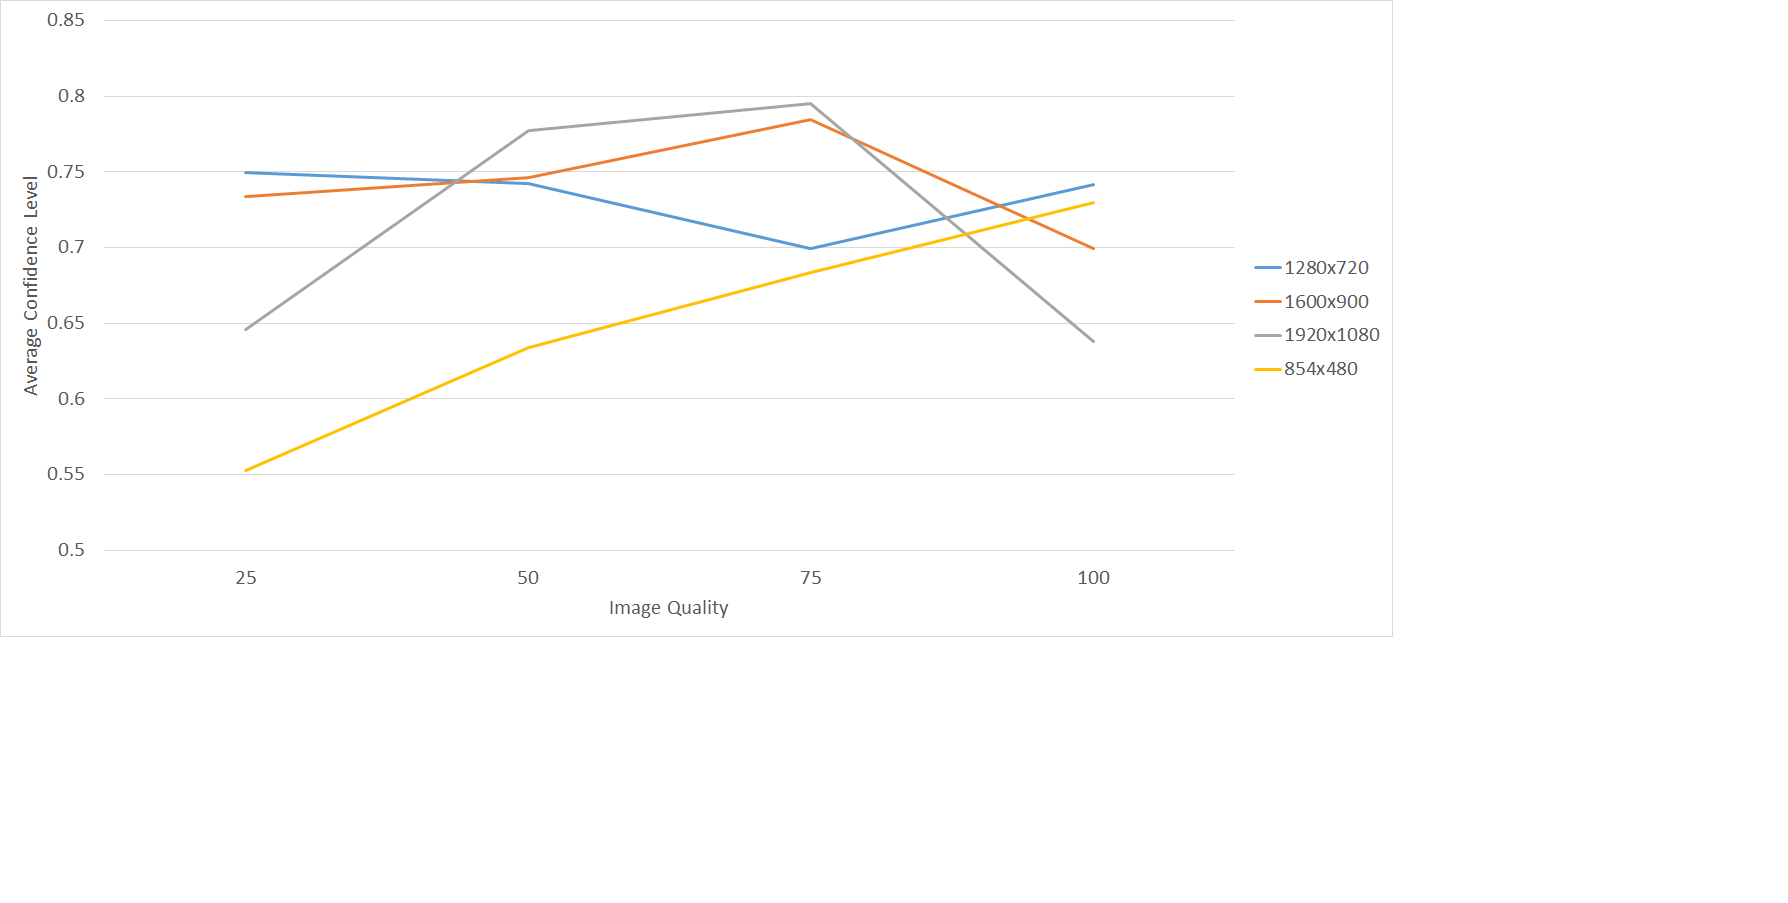
\includegraphics[width=\textwidth]{ImageResImpact}
\end{figure}

Given that these results were relatively inconclusive, and that the photos were not specifically suited towards the system's deployment scenario, a new batch of photos were created with the same settings but depicting the head and shoulder of a person. The exact labels and the values can be found in the Appendix (see \ref{ImageRecTesting}). Again, an average confidence level was evaluated and compared, and plotted as seen in Figure \ref{fig:ImageResImpactOnPerson}. Unfortunately, the results were not definitive or conclusive, but do similarly suggest a higher quality image aids service confidence. There is no clear advantage of one resolution over another, with both the low and high resolution photos performing poorly with low quality.

\begin{figure}[h]
\centering
\caption{Impact of Resolution and Compression on Service Response With Suitable Images\label{fig:ImageResImpactOnPerson}}
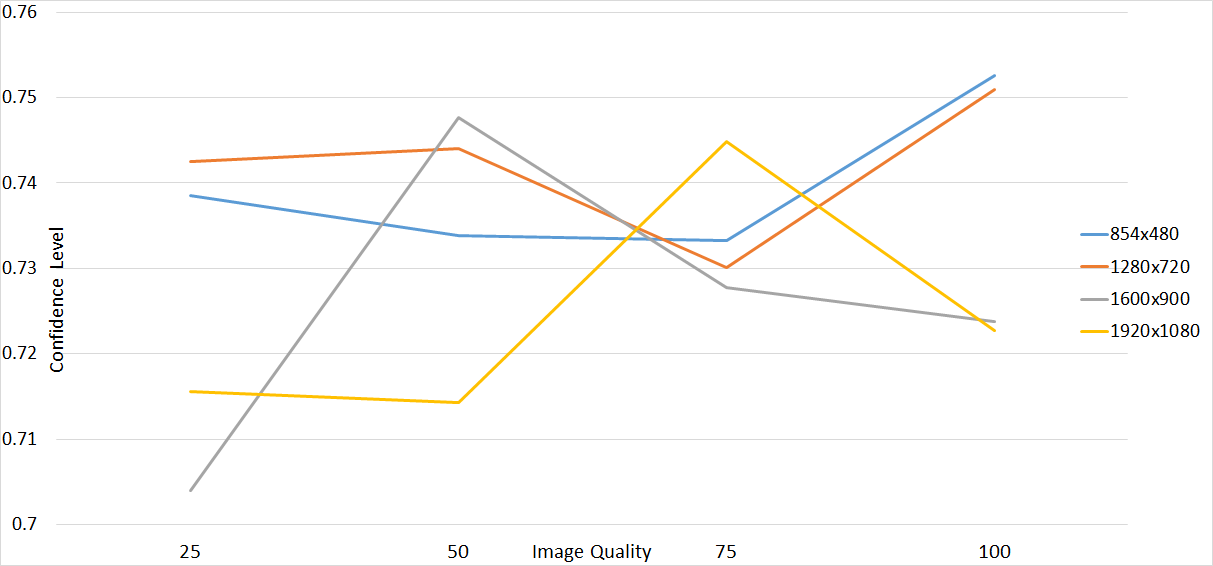
\includegraphics[width=\textwidth]{ImageResImpactOnPerson}
\end{figure}

\subsubsection{Other Variables}
By subtracting file upload time and recognition time from the total round trip time, we are able to determine the time between when an MQTT command is issued, and when the Pi receives it. Although the times measured did vary between 100 and 450ms and had high variance, there was no relation to the file which triggered the command. The average MQTT delay was evaluated as 251ms. This is a fixed latency that cannot be altered, and its relatively low value supports the use of MQTT to implement commands; a reasonable time between the Pi polling the server for commands added to the duration of the poll would be longer than 250ms. 

During the tests above, a command was sent as soon as service feedback was added. However, in a live system, there would be a delay of 0-1000ms, due to the time between the feedback arriving, and the DroneHandler detecting that it should change mode with its determineMode function, running on an interval of 1000ms. 







\subsection{Mocha}\label{mochaTesting}
Once a simple implementation of the server existed, the concept of testing to verify the implementation was considered. Whilst not engaging in pure Test Driven Development (TDD), testing is a vital part of this project to ensure the server behaves as it should, and that future expansions or improvements do not break the codebase or lead to unexpected behaviour. It proved very valuable throughout the project. Not engaging in pure TDD from the start turned out to be a suitable decision, as due to major reworkings of the server mechanics throughout the project many early tests would have been rendered useless. This was due in part to a developing knowledge and understanding of NodeJS and asynchronous code leading to a better solution, but a solution that was unfortunately incompatible with previous tests. 

The RESTful nature of the server, in that it should as much as possible be stateless, leans towards unit-testing. This means that each endpoint or item of functionality can be tested individually and independently. Indeed, the correct way to way to test a REST API is with a unit test\cite{mardan2014tdd}, and later in the project, TDD was employed for the support of the drone endpoints. The testing framework of choice was Mocha, as it is the industry standard for NodeJS; the majority of the modules used by this project are themselves tested with Mocha. Although other frameworks such as Jasmine\cite{jasmine} were considered, it is clear that Mocha is generally regarded as the most suitable for asynchronous NodeJS testing\cite{testingReview}. 

The Mocha framework was expanded with npm modules to verify the test, such as `should` and `assert` to ensure that the response is as expected. The Mocha framework works by running a set of described tests serially, with optional hooks before and after. Blocks of tests can be split up into suites. So for instance, a file upload test could run a before hook to login, run the test, and then run an after hook to delete any uploaded file. Initially, following a blog tutorial\cite{thewayofcode} the tests were run by creating a local instance of the server, and then executing the tests against the uri `http://localhost:8080/api/...`. However, when deploying to Bluemix this is not ideal, as in the Continuous Delivery Pipeline \ref{ContinuousDelivery} the tests are run in their own container from a single script. The `test` would therefore never end as starting a server instance is blocking. Without deploying an instance first, it would be difficult to test correctly. Therefore the module supertest was added, and the tests are run against a server object directly which is instantiated by Mocha, as described in the supertest documentation\cite{supertest}.

A small, somewhat simplified excerpt of Mocha testing can be found in the Appendix (see \ref{mocha1}. This snippet represents two tests, working on image endpoints. Before each test is run, an admin login occurs. This happens for every test so that they are independent; it should be possible to run just one of the tests and for it to succeed. The tests both run, with responses from the server matched against test values provided with `expect`. Any non-matching values throw an error. The after function is then called to remove any files that were uploaded.  

As well as testing the REST API, tests were made both for the functionality of the drone control and to ensure correct behaviour when given suitable stimuli. For instance, a test to check that when a sensor reading is uploaded it is saved to the database. The Scenario testing was to ensure that the system would react correctly to the scenarios defined in the Interim Report as part of the evaluation method. A small (modified) excerpt is included in the Appendix, showing a scenario test for fire (see \ref{mocha2}).

In this, Sinon spies and stubs are used\cite{sinon}. These are mock objects that can be used to monitor behaviour, by passing them as arguments to constructors. Here, mqttHandler has been defined as an object containing two spies, which is then passed to the \texttt{DroneCoordinator} constructor. Then, during test, if the \texttt{DroneCoordinator} module calls a function on the mqttHandler, the spy records this action. This can then be tested with assertions. The use of getModeNameWithDelay is due to how a \texttt{DroneHandler} changes its mode, as described in \ref{DroneControl}. The mode is changed at most once a second, with a delay of up to a second following suitable input. Therefore a delay of 1100 milliseconds is added before querying the mode that the drone is currently in.

If all API endpoint tests pass, and all unit tests and scenario tests pass, it can be assumed that the server would react as specified in the tests in-situ. Given that the specified behaviour directly relates to the scenarios from the Interim Report (see Appendix, Table \ref{scenarios}), the system satisfies the requirement to have this behaviour. However, this is only assessing the central section of system, not an end-to-end test. Full tests are described in ref{ImplementationTesting}

\subsubsection{Istanbul}
Code coverage is a measurement of the level of source code that is executed when a test suite is run. It is a core metric when evaluating a system and the effectiveness of its test, and was used as a tool in this project to ensure that as much of the codebase was tested as possible. The NodeJS module Istanbul was used to analyse code coverage, due to its ease of use, and well-formatted output\cite{istanbul}. This tool simply wraps around and runs Mocha, inspecting the code that is executed. A detailed HTML report is then generated, which shows exactly which lines of the codebase are executed, how many times, how many branches were taken, and so on. Istanbul was used as a technique to ensure that the testing was as comprehensive as possible. Figure CITE shows a snapshot of the output report from an Instanbul run. As can be seen, the test coverage is fairly high; the majority of the uncovered lines of code are for exception and error handling. Every time an external service is communicated with the error object returned must be checked, yet most of the time this object will be undefined so no action will be taken.

\subsection{Implementation Testing}\label{ImplementationTesting}
One of the most crucial type of test are full deployment tests, running the system end to end. This means once the system is running, closely inspecting the inputs and outputs to see if they match expectations. This nature of test were run regularly and repeatedly throughout the project. When an individual component, such as the server or Android, was developed and tested to work with sample input, the only way to test it completely is to run the whole system. However, due to the fact this covered such a wide range of components, there is no easy framework to run automated or quantitative tests. Therefore these were run on an ad-hoc basis. Videos of an Implementation Test can be found here //TODO on weekend. 

Implementation Testing inevitably highlights issues, some major, some minor, that can affect the correct functioning of the system. A select few are shown below, along with steps that were taken to rectify the issue.

\subsubsection{Multiple Dashboard Connections}
It became apparent that multiple dashboard (see \ref{Dashboard}) instances could connect to the server, but would not correctly receive all updates from the server - only one would receive data. This was found to be due to a break clause in the broadcast function on the server as it loops through all websockets clients. This was introduced to reduce broadcast time, but was removed due to it causing this issue.

\subsubsection{Erroneous Speech Transcripts}
Initially, any speech transcript returned from the IBM Speech To Text service were passed to the \texttt{DroneHandler}, which would enter InteractMode is the transcript was non empty. However, it was discovered that the service returned incorrect speech transcripts in an environment with background noise, which comprised purely of non-words such as `nnhm` which are presumably phonetic representations. The drone was therefore entering InteractMode needlessly and incorrectly, when no voice or person was present. To counteract this, a dictionary check was implemented. Each word in the transcript is checked against an English Dictionary file. Although any non-words could simply be removed, they may be useful for a user to identify missing words mid sentence. Therefore, a transcript is checked to ensure it contains at least one valid word, and if so the entire transcript is forwarded to the \texttt{DroneHandler}. 

\subsubsection{Image Label Confidence}
The feedback from the Image Recognition services is not particularly accurate or confidence. A suitable input would often not trigger a Mode change, due to the confidence score of a specific label not being high enough. Therefore, a dual trigger was implemented. A single label of high-confidence would trigger a Mode change as before, but in addition multiple image labels, whose confidence is above a lower threshold, could also trigger a mode change.

\subsection{Continuous Delivery} \label{ContinuousDelivery}
Continuous delivery is a methodology, whereby following a commit, the build, test, and deploy stages of a development lifestyle are automated. Automation, encompassing building, testing, and deploying, is not only time-saving, it can greatly increase the reliability of the code. The automatic flow of commit -\textgreater build -\textgreater test -\textgreater deploy means that no step can be skipped; if one step fails, the following steps are not executed. This means that the test step does not use existing executables if the build fails, and code which fails tests is not deployed. This, unsurprisingly, leads to more reliable code. As long as the build and test requirements are stringent enough, no `broken code` should ever be deployed\cite{co475}.

IBM devOps includes support for a continuous delivery pipeline. With this, a custom pipeline was setup. A git repository hosted by IBM acts as the starting point. When a push is made to this repository, it triggers a build phase, which for JavaScript is fairly simple and involves create a snapshot of the repository. This snapshot is passed to a test phase, which runs the Mocha tests specified above. Upon passing all specified tests, the snapshot is sent to a deploy stage, which installs all necessary packages and requirements to the Bluemix server, and deploys the application. 




\section{Results}

\subsection{Matching Desired Scenario Behaviour}\label{resultsScenarios}
In the Interim Report, a range of Scenarios (see Appendix Table \ref{scenarios}) were defined, with suitable trigger inputs and desired output actions. The range of output actions included commands for the drone, database interaction, and `raising a flag`, or sending a message, to the user. As described in the Mocha section(\ref{mochaTesting}), tests were written to ensure that the system behaves as expected. For testing these scenarios specifically, the test suite contained in Scenarios.js was written. This contains six sections, one for each scenario type, and are sub-divided again should there be multiple triggers for the scenario. 

In each test, the desired outcome is tested by using Sinon spies, with some or all of the checks below. The exact property or function tested varies (called, calledTwice, etc) depending on the exact scenario.
\begin{lstlisting}
 getModeNameWithDelay(function (result){
   assert.equal(result, "Interact", "Modes do not match"); // Ensure the drone is in the correct mode
   assert(mqttHandler.sendCommand.calledTwice, "MQTT Command not sent"); // Ensure the system sends commands to the drone
   assert(mqttHandler.sendEvent.called, "MQTT Event not sent"); // Ensure the system sends events to Android
   assert(sendUpdates.calledWith(droneName, 'event'), "sendUpdates not called correctly"); // Ensure the system sends event to the dashboard
   assert(cloudant.db.insert.called, "Database not used"); // Ensure the system logs the event to a database
   done();               
});
\end{lstlisting}

The system responds exactly to the scenarios defined, with two exceptions. `Explosion` is not triggered by a loud noise on the microphone. This is because the \texttt{DroneCoordinator} does not have access to the raw audio data. Whilst this could be relatively easily implemented, by passing the data and testing the maximum value against a threshold, this was not implemented due to time constraints and difficulty in assessing a suitable threshold value for an explosion. `Person in Distress` is not triggered by Tone Analysis feedback, as after testing the service it was deemed unsuitable for the project, as well as the fact that the concept of tone analysis is already employed in a simplistic manner by testing the audio transcript for key words.

Figure \ref{fig:MochaScenarios} shows the output of a successful Mocha test. Each line represents an individual unit test, with multiple lines under each scenario a different method of triggering the behaviour of that scenario, and therefore conformity to the desired behaviour that the system will be evaluated against. 

\begin{figure}[h]
\centering
\caption{Successful Testing of Scenarios With Mocha\ref{fig:MochaScenarios}}
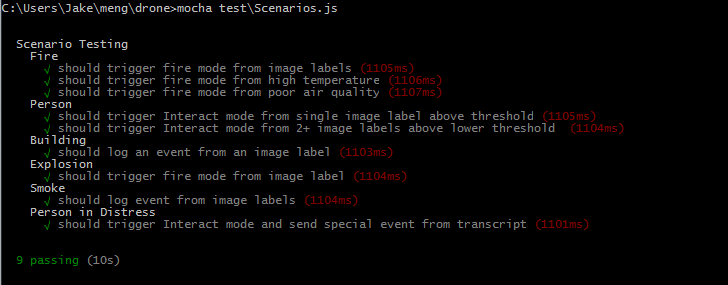
\includegraphics[width=\textwidth]{MochaScenarios}
\end{figure}

Due to the nature of the Mocha tests and Continuous Deployment, the server should always act as stated, as any alteration which changes system behaviour will be prevented from deploying by the automated testing.



\subsection{System Response Latency Estimation}
One of the most critical aspects of this system is the response time of the system end to end. This naturally is variable, though is most affected by two factors, file size and bandwidth from drone to server. Different types of data will have different latencies, due to the multiple channels of communication the drone uses to upload this data. Of interest here is the maximum latency, which is for the largest type of data, the file uploads. Other data types' latency is discussed below as well.

\begin{figure}[h]
\caption{Audio Recognition Duration with Varying File Size\label{fig:RecognitionDuration}}
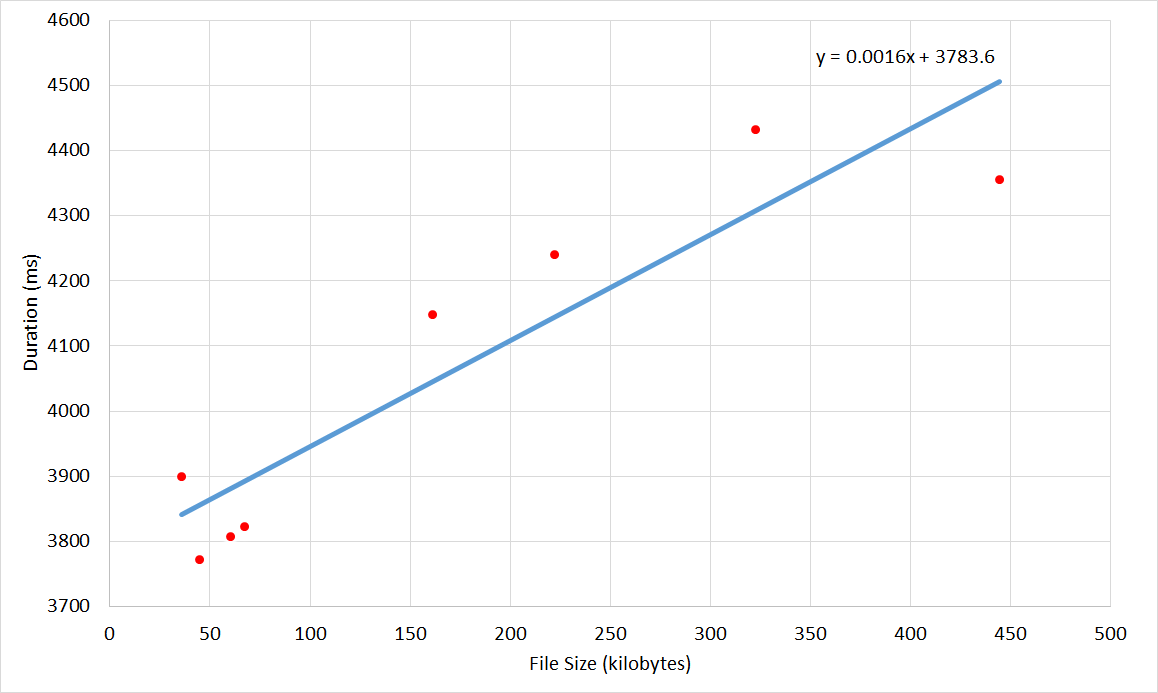
\includegraphics[width=\textwidth]{RecognitionDuration}
\end{figure}

Figure \ref{fig:RecognitionDuration} shows the increase in the delay of the audio recognition service as a function of file size. From this, a function can be generated to calculate the recognition delay given the file size. This, combined with knowledge of other parts of the system investigated in ref{LatencyBandwidth}, allows the latency time of the system to be determined as a function of average file size and bandwidth to the server, as represented below. All values that have been inserted have been measured through the tests in \ref{LatencyBandwidth}, and are assumed to be constant. Latency time and bandwidth are in seconds, and file size and bandwidth are in bits. This is to match the convention of providing bandwidth in bits per second. setMode delay is an average delay, the actual value can vary from 0 to 1. Although the value of $R$ is likely variable with file size, this is inseparable from the value of $B_r$, so has been left a constant with any change incorporated into $B_r$.

\begin{equation*}
\setlength{\jot}{10pt}
\begin{split}
Latency\ Time 	&= File\ Upload\ Time\ +\ Recognition\ Time\ +\ Command\ Time \\
				&= \frac{file\ size}{B_s} +\ \ \ R\ \ + \frac{file\ size}{B_r}\ +\ S\  +\ M \\
				&= \frac{file\ size}{B_s} +\ 3.784\ + \frac{file\ size}{5*10^6}\ +\ 0.5 +\ 0.25 
\end{split}
\end{equation*}

\begin{itemize}
	\item $B_s$ - Bandwidth to server
	\item $R$ - Recognition Service Constant Delay
	\item $B_r$ - Bandwidth from server to recognition service
	\item $S$ - Average Delay from setMode interval
	\item $M$ - MQTT Command Delay
\end{itemize}

This equation not only allows the user to gain an expected latency time for a system, but can aid in the system configuration. If a latency time below a certain threshold is desired, and the bandwidth to the server known, then the maximum file size can be determined. A maximum file size can determine the audio sampling or image resolution that is maximal without creating a longer than desired latency.

For example, if a maximum audio latency of 7.5 seconds is required, with a bandwidth to the server of 1Mbps, 

\begin{equation*}
\setlength{\jot}{10pt}
\begin{split}
7.5 	&= \frac{file\ size}{10^6} +\ 3.784\ + \frac{file\ size}{5*10^6}\ +\ 0.5 +\ 0.25 \\
2.966 &= \frac{file\ size}{10^6} + \frac{file size}{5*10^6} \\
2.966\ *\ 10^6\ *\ 5*10^6 &= file\ size\ *\ (10^6\ +\ 5*10^6) \\
\frac{2.966\ *\ 10^6\ *\ 5*10^6}{10^6\ +\ 5*10^6 } &= file\ size \\
 2471666&= file\ size\ (bits) \\
 308958 &= file\ size\ (bytes)
\end{split}
\end{equation*}

Given that the suggested maximum file size is around 300KB, and 16bit PCM wav file's size is $sampling\ rate*duration*2$ bytes, the user should consider reducing the default sampling frequency of 44.1Khz, or use mp3 files, otherwise the longest audio duration is less than 3.5 seconds. Note that audio can be greatly compressed via this method. A combination of using mp3s and reducing audio rate from 44.1Khz to 16Khz results in a file at least 10 times smaller, without a significant degradation of the service analysis.

The process above was repeated for the image files, with slightly different constants of $B_r = 13*10^6$ and $R = 3917$. Care should be taken when considering the bandwidth to the server, as both the audio and image uploads share the same bandwidth. Given the infrequency and very small size of MQTT messages, they can be deemed irrelevant. Additionally, if mp3 files are used, the average file size for potential upload is less than 10KB a second, even at 44.1Khz, whereas for images it is over 100KB for the most compressed image at the lowest resolution. Therefore the majority of the bandwidth should be dedicated to image upload.

\subsubsection{Maximum Latency Calculator}
Using the formula described above, a graph has been plotted with bandwidth against latency time, with a range of file sizes. This can be used as an aid by a user to help configure their system, as well as learning if a design change is needed; a higher bandwidth may be required. The graph is shown in Figure \ref{fig:LatencyVsBandwidth}. A similar graph with a larger Y axis range is located in the Appendix (Figure \ref{fig:LatencyVsBandwidthMaxAxis}), but here the range is reduced to increase spacing and therefore readability of the smaller latency values. 

In most situations, a user would want to maximise the quality of the data they upload, and therefore the file size, with the physical constraint of bandwidth and a virtual constraint of latency time, which may or may not be flexible. Note that the curves are near inverse exponential, due to the large constant factors in the equation. After a certain point, increasing the bandwidth does not significantly affect the system latency.

\begin{figure}[h]
\caption{Latency Calculator: Bandwidth Against Latency With Range of File Sizes\label{fig:LatencyVsBandwidth}}
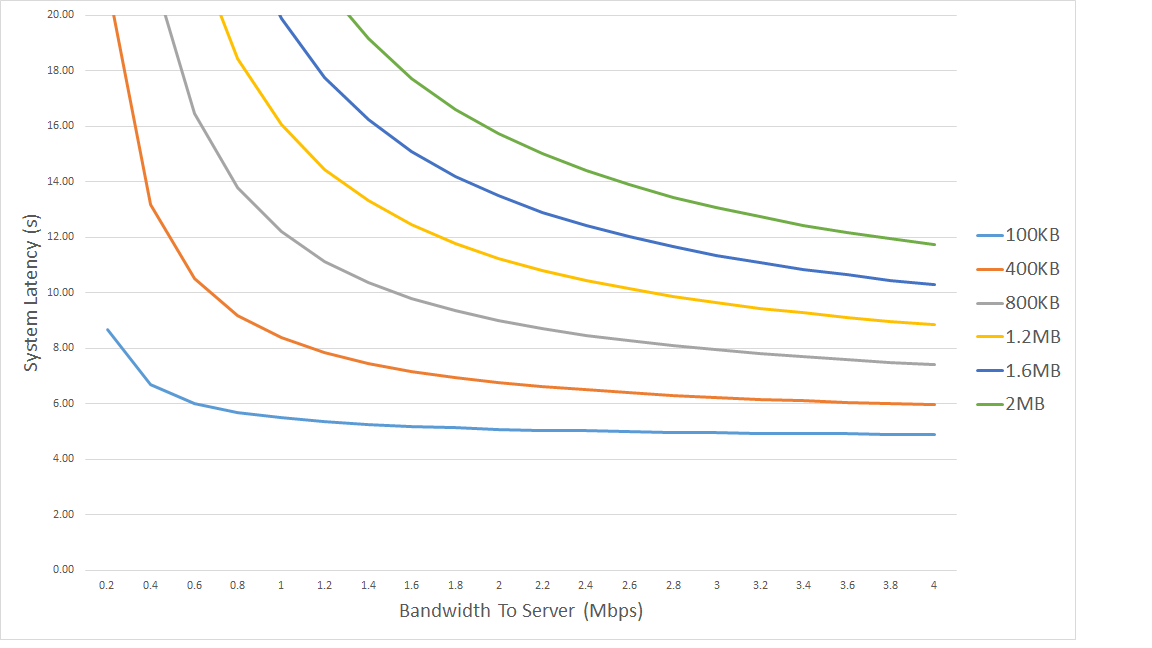
\includegraphics[width=\textwidth]{LatencyVsBandwidth}
\end{figure}

\subsubsection{Other Data Types' Latency}
As stated, the highest latency is for the large data files. The latency for a response from sensor data is much less. Given that the delay is twice the MQTT delay, plus the server analysis time, it can be calculated as below. As described above, the setMode delay is a value that can range from 0 to 1, so $0.5\pm0.5$ is used.

\begin{equation*}
\begin{split}
Latency\ Time\ For\ Sensors & = MQTT\ Delay + setMode\ Delay + MQTT\ Delay \\
							& = 0.25 +\ \ 0.5 \pm 0.5 \ \ + 0.25 \\
							& = 1\ second \pm 0.5 \\
\end{split}
\end{equation*}

\subsection{Scalability}
One of the system requirements of the system is that although it only needs to be implemented for one drone, thought should be given to scalability, with the idea of supporting drone swarms in the future. Needless to say, the fact that the drone can support concurrently multiple drones proves that this was done with great success. Although only tested with 3 drones, scaling to greater drone number should be seamless until hardware limits are met. These are namely those of the server, both in terms of its bandwidth and ability to handle multiple requests. 

Approaching these limits, server performance will likely diminish without being rendered unusable. With three drones attached, there was no noticable impact on the server latency as described above. 

Through virtue of the nature of NodeJS, many concurrent connections can be handled simultaneously, as a new connection does not create a new thread as is the case in many other web servers. However, this does mean that whilst the single NodeJS thread is executing no other requests or existing connections can be handled. There is therefore a limit, especially for this system where the thread has computational background tasks such as the drone control. Even though this is running simple fast switch statements, for many drones this may cause the server to refuse requests. More threads are needed.

There are two methods to increase the number of threads; NodeJS clustering and increasing the number of servers. NodeJS clustering is a concept where multiple and usually identical node threads are executed concurrently. Inter-thread communication is possible through NodeJs `events`, or even through TCP. Both methods present the same problem, that of consistency. The API, with the exception of websockets, is completely stateless. This means that it makes no difference which thread a drone connects to. However, for websockets and DroneControl, state information is saved on the server. This means that if a drone connects to a different thread than previously, there would be system inconsistency.

This inconsistency can be managed in three ways. Firstly, whilst multiple threads to handle stateless API actions could be created, a single thread with state information is used. Due to the modular nature of the codebase, separation would be relatively simple. If multiple servers are used, this could be a central server which all others connect, in a similar manner to the other IBM cloud services. Secondly and more complexly, multiple threads with state information can run, communicating any changes in state with each other. Conflict resolution will be required. Whilst the first is simplest, the second could be made to be more robust. A third solution is to have a load-distributing thread which all connections are made to, which then acts to simply forward all requests from a single drone to a single thread to ensure consistency. 

The bandwidth is a fixed connection from the server, and cannot be increased unless a bigger bandwidth is paid for, or increasing server number as described.


\section{Evaluation}
In this section, the project is implemented against two criteria; how well it matched requirements and specification, and how suitable the concept of using cloud services to aid data analysis in a search and rescue situation is when compared to alternatives.
 
\subsection{Testing of situations}
The primary method of assessing project success is by verifying that the created system acts in the desired manner, aided by cloud services. To evaluate this, a range of scenarios were created, as detailed in Table \ref{scenarios}. Not only did they describe desired behaviour in line with the Requirements Capture, they contained drone flight commands. Whilst development did focus around these specific scenarios, it was ensured that the system's architecture supported behaviour additions, to match alternative scenarios easily. This was implemented through the modular design of the drone control.

For each scenario, the system was tested to ensure it exhibited the desired behaviour. On the most important and extensive component, the central server, this testing was in the form of Mocha tests (see \ref{resultsScenarios}). The conformance of the other components was ensured by running end-to-end tests with sample inputs, and inspecting resultant behaviour. The final implementation successfully pasts all test, meeting the requirement. 

Whilst this kind of behaviour could be adopted for onboard processing, having this functionality in the cloud is more flexible; a new behavioural trait can be added at a single point to affect all drones. This can even be done whilst the drones are in the air, providing the server restart time was sufficiently brief, and does not require a connection to the more difficult to alter software on the small devices.

\subsection{Latency}
The main quantitative metric for evaluating this system was the system latency response. System response is an important factor in search and rescue where time is of the essence. This was found through testing to be:
\begin{equation*}
\setlength{\jot}{10pt}
\begin{split}
Latency\ Time 	&= File\ Upload\ Time\ +\ Recognition\ Time\ +\ Command\ Time \\
				&= \frac{file\ size}{B_s} +\ \ \ R\ \ + \frac{file\ size}{B_r}\ +\ S\  +\ M \\
				&= \frac{file\ size}{B_s} +\ 3.784\ + \frac{file\ size}{5*10^6}\ +\ 0.5 +\ 0.25 
\end{split}
\end{equation*}
However, it was found that the majority of factors within this formula are uncontrollable. Recognition time cannot be changed, and file upload time is dependent on the bandwidth and file size. Bandwidth available is often related to money; a better financed solution can afford more expensive hardware and a higher bandwidth. For this project, the fastest easily available internet connection, 4G, was used in the field, whilst existing domestic internet was used for development and testing. There was therefore no easy way this could have been increased any further. The value of $M$ was an uncontrollable constant, yet is a suitably low value. 

The only completely implementation dependent value is that of $S$. This is an easily configurable value by changing the interval of \texttt{setMode} as described in \ref{DroneControl}, with the current value a medium between system latency and availability. File size was controllable, and techniques to minimize size whilst maintaining system accuracy were investigated. 

Whilst much of the latency cannot be altered, the system implementation does not add a great amount to the base value, and can be configured to adapt to different connections. A latency time of 10 seconds can be deemed short enough for a deployed system, with the system therefore satisfying original requirement to minimise latency. 

The latency times of cloud services and onboard processing are comparable. Cloud services introduce a communication latency, whilst onboard processing takes longer due less computational power. Concrete values for comparison fluctuate greatly, dependant on the exact implementation and level of optimisation. Of interest for future development is the geographical location of the cloud services. Inspecting the IP addresses of the IBM analytical services revealed them to be located in the USA, a long distance from the system deployment. It is likely that a UK or European implementation of the cloud services would greatly reduce the system latency.


\subsection{User Interface}
The final requirement of the project was to provide the user with resultant information and analysis from the system. This was achieved in more than one way. The simplest and most information dense method is inspecting server logs, which are made available through a URI. However these are very long streams of text logging every action of the server, and are not suitable for any use other than debugging. 

The primary feedback method throughout the project was that of the Android app, detailing both raw data and analytical results. These results were presented in both quantitative and qualitative manners, to provide the user with a user-friendly interface whilst still allowing access to exact values.

The secondary feedback method of the Dashboard was only implemented as a very brief expansion, yet has greater functionality than the Android app. Similarly, it can show data quantitatively and qualitatively. The Dashboard additionally has the Settings section, allowing user control of the system as well as viewing feedback. Due to the nature of larger screens used to view the Dashboard, all this information can be displayed on one page unlike the Android app, which leads to a much better user experience. 

The existence of many of the API endpoints provides access to legacy data, rather than just live data. Although the focus of the system is of course on live data, reviewing past flights could lead to insights and system improvements, as well as informing the user. The only use of these within this system implementation is to view legacy images on the Dashboard, or to view legacy sensor data on the Android app.  

The project meets the requirement to provide the user with feedback from the system, and does so in a variety of informative and easy-to-understand ways. However, given the rate of development of the Dashboard, the choice of implementing an Android App as explained in \ref{Feedback} was perhaps poor. Although more thought could have been to development time, this was a difficult task. There was a lack of experience in both web development and Android, so both would require a steep learning curve with an unknown speed of development. However, once it was realised that web development was much quicker, the dashboard rapidly gained the same functionality as the Android app, and surpassed it. 

The use of cloud services is most noticeable in this section of the project. Onboard processing would only provide a user with data through flight logs, inaccessible during system use, or through direct communication. The advantages of cloud services are many, allowing legacy data inspection (Cloudant), live dashboard and API (NodeJS server) which would be too `heavy` for a drone to support mid-flight, and remote connections (MQTT and HTTP). However, some of these advantages also apply to a local ground station such as described in \ref{PotentialSolutions}.


\subsection{Connection Requirements and Dependency}
For cloud services, an internet connection is required. Although this system has been built to be robust to intermittent and relatively slow internet connections, it still requires some degree of connectivity. This may not always be achievable in remote areas, especially in a search and rescue situation caused by a natural disaster which may disrupt infrastructure. This is a serious negative for the use of cloud services, and is the primary drawback when compared to onboard processing. 

Given that this requirement stands, this project has aimed as much as possible to deal with poor connectivity, by handling loss of HTTP or websocket connections, and through the use of the MQTT service rather than a simple `fire and forget` protocol. 

A secondary drawback is dependency on external services which are outside of a user's control. This was an issue numerous times throughout the project; at various points the Cloudant database, SQL database, or even the entire Bluemix PaaS were unavailable for extended periods of time. This leads to a critical failure to the system, and is obviously completely undesirable for search and rescue. This is an issue which can only be solved by using paying services which are likely to be more reliable, or incorporating redundancy and duplicate services from different vendors.  


\subsection{Analytical Services}
Through testing of the analytical services, the content, accuracy and confidence of the responses is currently unsuitable for a real system deployment. The responses are highly variant, leading to many false positives if system criteria are too lax, and false negatives if too strict. Neither of this situations is suitable for search and rescue. Receiving false positives from multiple drones will swap rescuers with information, wasting time. False negatives are completely unacceptable, as they could lead to a casualty or situation being overlooked.   

Despite these drawbacks, analytical cloud services are likely to give much better results than onboard implementations. The concern is with the current level of machine learning methods rather than a case of where the algorithm should be executed. This will improve with time.

\subsection{Project Approach}
\subsubsection{AGILE Methodology}
The AGILE approach to this project was explained in \ref{AnalysisAndDesign}, and with hindsight was the correct methodology to have used. With more than one interdependent component, it can be difficult to develop one part if another is not functioning correctly. Frequently ensuring that all components worked correctly and developing with incremental changes meant that new functionality could be tested as soon as it was written. Inspecting the Git history of each repository highlights this, as in Figure \ref{fig:GitAnalysis}. A Git addition represents a single line of code that has been changed. Barring plateaus during Easter exams and break, every component was continually developed concurrently, although it is noticeable in the last two weeks when development of the dashboard in the Drone repository took preference over the slower-to-develop Android App. This again proves the benefits of the AGILE methodology, being able to react changes seamlessly.

\begin{figure}[h]
\centering
\caption{Cumulative Git Additions For Each Repository\label{fig:GitAnalysis}}
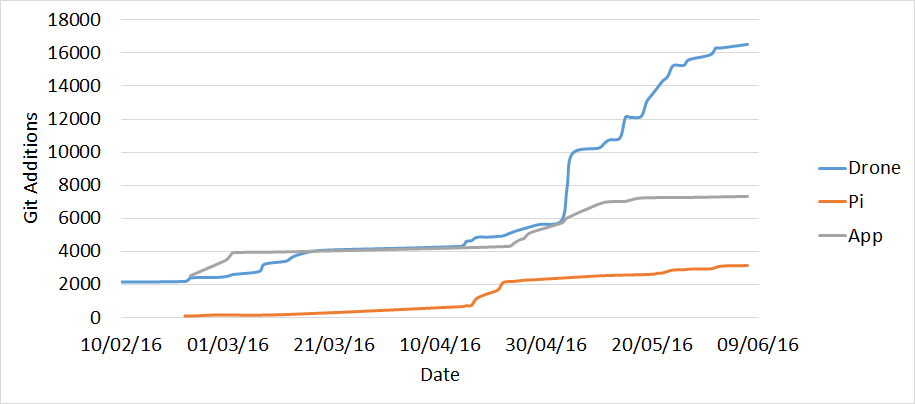
\includegraphics[width=\textwidth]{GitAnalysis}
\end{figure}


\subsubsection{Review}

//From Jon

\subsection{Summary}
All original project objectives were met, as described above. A system was created that was capable of using cloud services to aid in the analysis of data collected by a drone, and feed this back to a user. However, due to the dependency on cloud services it has significant disadvantages when compared to alternative research into onboard processing. These are mainly related due to the dual factors of an internet connection, both as a requirement and additional response time, and the not yet ideal response from analytical cloud services. 

The project focus was on functionality and proof of concept. Therefore, while some steps have been taken to ensure that the system is robust, the system is not durable enough to be used in a real situation. Unexpected exceptions will cause the system functionality to be reduced. On a Python thread this may only halt a single aspect of data collection, but an unhandled server exception would cause system failure. However, time was instead spent upon increasing server functionality and characteristics. 

Due to the flexible nature of the project requirements, this reduction in durability provided the chance to implement practices that resulted in a much more comprehensive and complete development process and resulting solution. System security is not considered as part of the project requirements or specification, yet has become a very interesting and challenging aspect of development. Conversely, the use of continuous delivery was a simple concept and relatively easy to implement, and simplifies the deployment workflow greatly. Automated testing with the Mocha framework is another example of learnt skills being applied to enhance project functionality, and to some degree aids the durability of the system, although further mocking of remote services to allow failure testing would be required to have a great impact.

Due to the focus of the system upon cloud services and not onboard processing, little consideration has been given to optimising the Raspberry Pi software. Focusing on ease of development, this works with many threads upon a single cored machine, in a relatively slow scripting language. It is likely that with a newer, more energy-efficient Raspberry Pi with four cores, a conversion from Python to C, and streamlining of existing algorithms, that a reasonable amount of CPU power should become available for onboard processing.

To summarise, this project has succeeded in creating a system which utilises cloud services to aid drone use in search and rescue, but that the system is not yet ready for use. In the short term this is an issue of making the system more robust and durable. In the long term, this is a concern of awaiting machine learning and analytical cloud services to improve until resultant analysis is more refined and accurate.

\section{Conclusion}

The use of cloud services for aiding data analysis in a search and rescue environment is a practical solution for reducing search time. However, although this system demonstrates that the solution is viable and could be implemented, further work is needed on analytical cloud services before a system could be used. 

Although a latency time of 10 seconds is acceptable, it is not ideal. This is not in terms of absolute time, but is related to the fact that the drone will have moved during this time. A command to stop the drone will stop it 10 seconds away from the trigger event, which depending on drone speed could be a considerable distance. Design choices throughout the project's development aimed at reducing this time through asynchronicity and concurrency.

However, the major issue discovered in this project was suitability of response content from cloud services. Image Recognition services did not return a great variety of suitable labels, and the often returned completely incorrect labels. Even for ideal input images, a response did not have a high level of confidence. There is potential to improve the response of services, through training and enhancements. However, improvement of the services is beyond the scope of this project, and can only be achieved by IBM. 

Nevertheless, this system can support a small fleet of drones, which if preprogrammed with routes could collaboratively cover a large area in a fraction of the time manual human inspection would take. This could, with further development, become a valuable tool in a search-and-rescue situation. 

The difficulties faced in this project mostly revolved around the steep learning curve and subsequent complexity of the system. This system was built with very little prior knowledge of the software techniques and hardware used. A number of skills and techniques were learnt, as well as a large knowledge base. As well as new information, skills that had been learnt previously were used to create an enhanced system, which complies with multiple industry standards, as well as being secure and well documented. The complexity was managed through modular additions and improvements, and constant testing of correct functioning.

It is likely that a future implementation will use a mixture of onboard processing and cloud services, to gain the advantages of both and eliminate the challenges faced when only using one. In terms of this system, it met every specification goal and requirement, going beyond what was necessary in many aspects to result in a well designed, complex and viable system with potential for future development.

\section{Future Development}
Although the primary aspect of the system which needs to be improved is the quality of the remote cloud services, there are many areas of the system which can be developed upon to improve its viability as a solution. Indeed, some of these are planned to be implemented by IBM following the completion of the project. Some of the following suggestions have already been attempted or started, but are contained within this section due to no actual working implementation.

\subsubsection{Drone Control And Handling}
The server has a structural framework supporting much greater control of the drone and interpreting the service analysis than is implemented. As described in \ref{DroneControl}, the modular approach to controlling the drone allows high customisation. The \texttt{DroneHandler} can be altered to affect which mode it enters and when, by changing how it interprets its \texttt{modeFactors} object. Custom modes can be easily added, inheriting from the base or normal, which can change how data is handled. For example, a custom mode designed for interaction could inspect an audio transcript in more detail, acting upon the words. 

\subsubsection{Improving Input Data}
The data which is passed to the services is, in the current system implementation, raw and unfiltered. It is possible that some data manipulation before passing them to the service would improve the quality of the response. This is specifically relevant for the audio services. As shown in \ref{testSpeechRec}, the Speech To Text service is noise susceptible. It is possible that some digital signal processing could be implemented, either on the Raspberry Pi or the server, to minimise the noise level.

Similarly, some simplistic image recognition could be implemented onboard the Pi, to determine whether an image is worth sending to the image recognition service. An example may be ensuring that the colour difference across the image is great enough, as with no differentials the service may generate meaningless responses. This would reduce the bandwidth required by the system.

\subsubsection{Improving Output Methods} \label{OutputMethods}
The drone can become more versatile by expanding its output methods. A primary example is that of speech or text output, from a speaker or a screen. This is largely already implemented for speech; the server has a pair of websockets for transmitting audio to the drone, and the drone can correctly receive this audio. However, there is no playback hardware currently connected to the drone, although the existing 3.5mm jack and command-line audio player `aplay` mean this is a trivial issue of connecting a speaker, and adapting a thread to run the `listen` function in audioCapture.py. Likewise, a text display would be a relatively trivial operation of attaching the screen, and parsing a PiCommand to output text. 

\subsubsection{Onboard Decisions}
Some of the commands that the server generates are triggered by threshold checking of simple data such as sensor readings. This does not need any cloud services or server support, and could be entirely implemented on the board itself, which then notifies the server of the decision. This was not implemented in this project as it was focussing on doing as much as possible in the cloud, but in a deployed system this should be implemented to reduce communication levels and response times. 

\subsubsection{More Cloud Analysis}
Some IBM analytical services were not used due to their inaccurate responses, while others have input that this system doesn't provide, such as large bodies of text. These services will undoubtedly improve over time, due to the fact they are based on machine learning algorithms. Once they become viable, they can be added to the system.
 
\subsubsection{Expansion of the Dashboard}
The Dashboard proved to be a component that was capable of rapid development, and could handle advanced aspects of the system such as live and real-time configuration changes. This could have been developed much further, providing the functionality to plan autonomous drone flights, set way points mid flight, and otherwise interact with the system to a greater capacity. An interesting addition would be that of stream audio back to the drone, for use as mentioned in \ref{OutputMethods}.

\subsubsection{Autonomous Flight}
Although the autopilot is capable of navigating through waypoints, it has no surroundings awareness or collision avoidance. For example, SLAM modelling could be implemented, or even simple distance sensors could be used to aid drone flight. Use of set-distance infra-red interrupters was attempted, but these were far too inaccurate; full distance sensors would be required. 

\section{User Guide}\label{UserGuide}
Each of the three main components, the drone, server and app, each have their own git repository, containing all source code. Each has a README.md describing installation steps for use, including required dependencies, and basic usage. 

The Raspberry Pi requires a Raspbian (or similar Debian) operating system running, and then the exact steps can be followed for installation and execution.

The Server describes numbered installation steps, but some these are directions to websites with platform specific installation instructions, such as for NodeJS

The Android App requires a more extensive toolchain for compilation than the other two repositories. For ease, the integrated development environment (IDE) Android Studio by Google is suggested as the method for development and installation. The Android Studio project files are provided for easy IDE configuration. Again this is platform specific, so instead of providing instructions a link is provided to the Android developer's website. Any dependencies or required modules should be installed by Android Studio, either automatically or through installation wizards and prompts. 


The repositories are available at: 
\begin{itemize}
	\item Pi software: \url{https://github.com/jake2184/drone_pi}
	\item Server Software: \url{https://github.com/jake2184/drone}
	\item Android App: \url{https://github.com/jake2184/drone_app}
\end{itemize}

The system is largely automatic, therefore once running there is little need for user guides or interaction. For the server, there is documentation available detailing both the external API for any client, and also the internal functions for a future developer. 




\section{Appendix}

\begin{table}[h]
\caption{Search and Rescue Scenarios\label{scenarios}}
\hyphenchar\font=-1
\centering
\begin{tabularx}{\textwidth}{| >{\centering}m{1.5cm} | >{\centering}m{2cm} | X | X |}
    \hline
    Name & Description & Trigger & Action \\ \hline
    Fire & \vspace{\baselineskip} A fire is present &
    \begin{itemize}[topsep=0pt, leftmargin=0cm,itemindent=.5cm,labelwidth=\itemindent,labelsep=0cm,align=left]
        \item Image Recognition returning a related label, such as “Wild\_Fire”
        \item Temperature sensor recording an abnormal temperature, eg >40C
    \end{itemize} &
    \begin{itemize} [topsep=0pt, leftmargin=0cm,itemindent=.5cm,labelwidth=\itemindent,labelsep=0cm,align=left]
        \item Send avoidance movement commands to the drone, such as to increase altitude
        \item Raise flag, log occurrence and location of drone
    \end{itemize} \\ \hline

    Person & \vspace{\baselineskip} A person is present &
    \begin{itemize} [topsep=0pt, leftmargin=0cm,itemindent=.5cm,labelwidth=\itemindent,labelsep=0cm,align=left]
        \item Image Recognition returning a related label, such as `person', `adult', `child'
        \item Speech to Text returning a viable result
    \end{itemize} &
    \begin{itemize} [topsep=0pt, leftmargin=0cm,itemindent=.5cm,labelwidth=\itemindent,labelsep=0cm,align=left]
        \item Halt movement of drone to allow operator to act suitably
        \item Raise flag, log occurrence and location of drone
    \end{itemize} \\ \hline

    Building & \vspace{\baselineskip} A building is detected &
    \begin{itemize} [topsep=0pt, leftmargin=0cm,itemindent=.5cm,labelwidth=\itemindent,labelsep=0cm,align=left]
        \item Image Recognition returning a related label, such as “Rural\_Building”
    \end{itemize} &
    \begin{itemize} [topsep=0pt, leftmargin=0cm,itemindent=.5cm,labelwidth=\itemindent,labelsep=0cm,align=left]
        \item Log occurrence, attempt to log location of building
    \end{itemize} \\ \hline

    Explosion & \vspace{\baselineskip} An explosion has occurred &
    \begin{itemize} [topsep=0pt, leftmargin=0cm,itemindent=.5cm,labelwidth=\itemindent,labelsep=0cm,align=left]
        \item Image Recognition returning a related label, such as “Explosion”
        \item A sudden large noise on the drone microphone
    \end{itemize} &
    \begin{itemize} [topsep=0pt, leftmargin=0cm,itemindent=.5cm,labelwidth=\itemindent,labelsep=0cm,align=left]
        \item Halt movement until operator can act suitably ie move drone away, or the Fire scenario occurs
        \item Raise flag, log occurrence
    \end{itemize} \\ \hline

    Smoke & \vspace{\baselineskip} Smoke is present &
    \begin{itemize} [topsep=0pt, leftmargin=0cm,itemindent=.5cm,labelwidth=\itemindent,labelsep=0cm,align=left]
        \item Image Recognition returning a related label, such as “Smoke”
    \end{itemize} &
    \begin{itemize} [topsep=0pt, leftmargin=0cm,itemindent=.5cm,labelwidth=\itemindent,labelsep=0cm,align=left]
        \item No avoidance needed, indeed smoke may be a useful marker to investigate
        \item Raise flag, log occurrence
    \end{itemize} \\ \hline

    Person in Distress & \vspace{\baselineskip} A person is in need of assistance &
    \begin{itemize} [topsep=0pt, leftmargin=0cm,itemindent=.5cm,labelwidth=\itemindent,labelsep=0cm,align=left]
        \item Speech Recognition transcript containing key words, such as `help` or `danger`
        \item Tone Analysis returns analysis indicating stress, anger or a request
    \end{itemize} &
    \begin{itemize} [topsep=0pt, leftmargin=0cm,itemindent=.5cm,labelwidth=\itemindent,labelsep=0cm,align=left]
        \item Further to action of scenario `Person`, the request should be forwarded to a relevant display device
        \item Raise flag, log occurrence
    \end{itemize} \\ \hline


\end{tabularx}
\end{table}



\subsection{SQL Table Definitions} \label{SQLDefinitions}
\begin{center}
\begin{lstlisting} 
CREATE TABLE "USERS"
(
  "username" VARCHAR(20) NOT NULL,
  "first_name" VARCHAR(20),
  "last_name" VARCHAR(20),
  "salt" VARCHAR(8) NOT NULL,
  "password" VARCHAR(64) NOT NULL,
  "role" INT NOT NULL,
  CONSTRAINT "primary_key" PRIMARY KEY ("username")
) ORGANIZE BY ROW;


CREATE TABLE "DRONES"
(
  "name" VARCHAR(20) NOT NULL,
  "model" VARCHAR(20),
  "owner" VARCHAR(20) NOT NULL,
  CONSTRAINT "primary_key" PRIMARY KEY ("name"),
  CONSTRAINT "owner_key" FOREIGN KEY ("owner") REFERENCES USERS("username")
) ORGANIZE BY ROW;
\end{lstlisting}
\end{center}

\subsection{REST API} \label{apdxRestApi}
\subsubsection{Sensors}
\begin{center}
	\begin{lstlisting}
		GET /api/:dronename/sensors
		GET /api/:dronename/sensors/:timeFrom
		GET /api/:dronename/sensors/:timeFrom/:timeUntil
		GET /api/:dronename/sensors/:timeFrom/:timeUntil/:type
	\end{lstlisting}
\end{center}
The sensors api endpoints are designed for the querying of historical data. They take a range of path parameters and return a JSON array of the relevant documents contained in the database. The primary use within this project is for the Android app to query and plot legacy data. The app has developed to now only use the longest sensor endpoint, but the rest are kept for completeness. This will, as is self-evident, return documents relating to a specific drone between a time window and of a certain type. Whilst URI query parameters rather than path parameters could have been used, this was avoided to ensure a more standard and simplistic API where as much as possible is defined in the path. A typical query would be `GET /api/pixhack/sensors/1465231987452/1465231997452/temperature`.

\subsubsection{GPS}
\begin{center}
	\begin{lstlisting}
		GET /api/:dronename/gps
		GET /api/:dronename/gps/:timeFrom
		GET /api/:dronename/gps/:timeFrom/:timeUntil
	\end{lstlisting}
\end{center}
The gps endpoints are very similar to the sensors endpoints, but simply query the positionlog rather than the sensorlog database. The information should also be present in the sensorlog database, but this provides a lighter weight access point for position data, for instance for plotting historical routes. A typical query would be `GET /api/pixhack/gps/1465231987452/1465231997452`.


\subsubsection{Images}
\begin{center}
	\begin{lstlisting}
		GET    /api/:dronename/images
		GET    /api/:dronename/image/:docID
		POST   /api/:dronename/image/:docID
		DELETE /api/:dronename/image/:docID
	\end{lstlisting}
\end{center}
The images endpoints are for file handling. Similar to the sensors endpoints, they can be used to obtain historical files, but also for file upload and deletion. These endpoints have two main uses within the project. Due to large files being unable to be transferred over MQTT, a HTTP method is required. Indeed, this is one of the reasons that the system has this REST API. The drone uses the POST method to upload captured image files, whilst the Android client uses the GET endpoint with the docID `latest` to retrieve the latest image. A typical query from the client would be `GET /api/pixhack/image/latest`, and from the drone would be `POST {'image':@1465231987452.jpeg} /api/pixhack/image/1465231987452`, as well as the body containing metadata such as the GPS location of the image. 

\subsubsection{Audio}
\begin{center}
	\begin{lstlisting}
		GET    /api/:dronename/audio
		GET    /api/:dronename/audio/:docID
		POST   /api/:dronename/audio/:docID
		DELETE /api/:dronename/audio/:docID
	\end{lstlisting}
\end{center}
The first set of audio endpoints are similar to the image endpoints, for file transfers from the drone and to a client. They work in a very similar way, although there is currently no component of the system that requires any audio file to be fetched from the database. 
\begin{center}	
	\begin{lstlisting}
		WS /api/:dronename/audio/stream/listen
		WS /api/:dronename/audio/stream/talk
		WS /api/:dronename/audio/stream/upload
		WS /api/:dronename/audio/stream/download
	\end{lstlisting}
\end{center}
This set of endpoints are websockets. These supply two audio streams for each drone; one (upload/listen) collects audio from the drone and broadcasts it to the listeners, and the other (talk/download) does the opposite. Having 4 end points, rather than two or even one, allows easy isolation of the data which can therefore be sent as pure binary audio, and means the scripting on the drone can have two separate threads to listen or send, preventing any issues with resource blocking. These were implemented to satisfy the evolving requirements of the system. 


\subsubsection{Users}
\begin{center}
	\begin{lstlisting}
		GET    /api/users/:username
		POST   /api/users/:username
		DELETE /api/users/:username
	\end{lstlisting}
\end{center}
The users endpoints are primarily for admin management of user accounts stored in the SQL database. Individual accounts can be created, queried, and deleted. User accounts are crucial to the api. Without a user account and subsequent cookie, a client cannot do any action on the api. These endpoints are more restrictive than the others. Only an ADMIN can POST a new user, and only an ADMIN or the user themself can GET or DELETE a username. 

\subsubsection{Drones}
\begin{center}
	\begin{lstlisting}
		GET    /api/drones
		POST   /api/drones
		DELETE /api/drones/:dronename
	\end{lstlisting}
\end{center}
The drones endpoints are for management of registered drones in the SQL database. A user can request a list of their drones with a GET request, POST a new drone, or DELETE an existing drone. The creation and deletion of drones from the SQL database cascades to the Cloudant database, creating or deleting all relevant databases. The cookie values are used to identify the user for drone endpoints, and are incorporated into the SQL queries, restricting access for any client to their own registered devices. 


\subsection{Android Fragments}
Figure 9 shows a selection of screenshots from the Android app. These were taken around a minute after the drone established a connection.
\begin{landscape}
\begin{figure}[h]
\caption{Screenshots of the Android App\label{fig:AndroidScreenshots}}
\centering
\begin{subfigure}[b]{.45\linewidth}
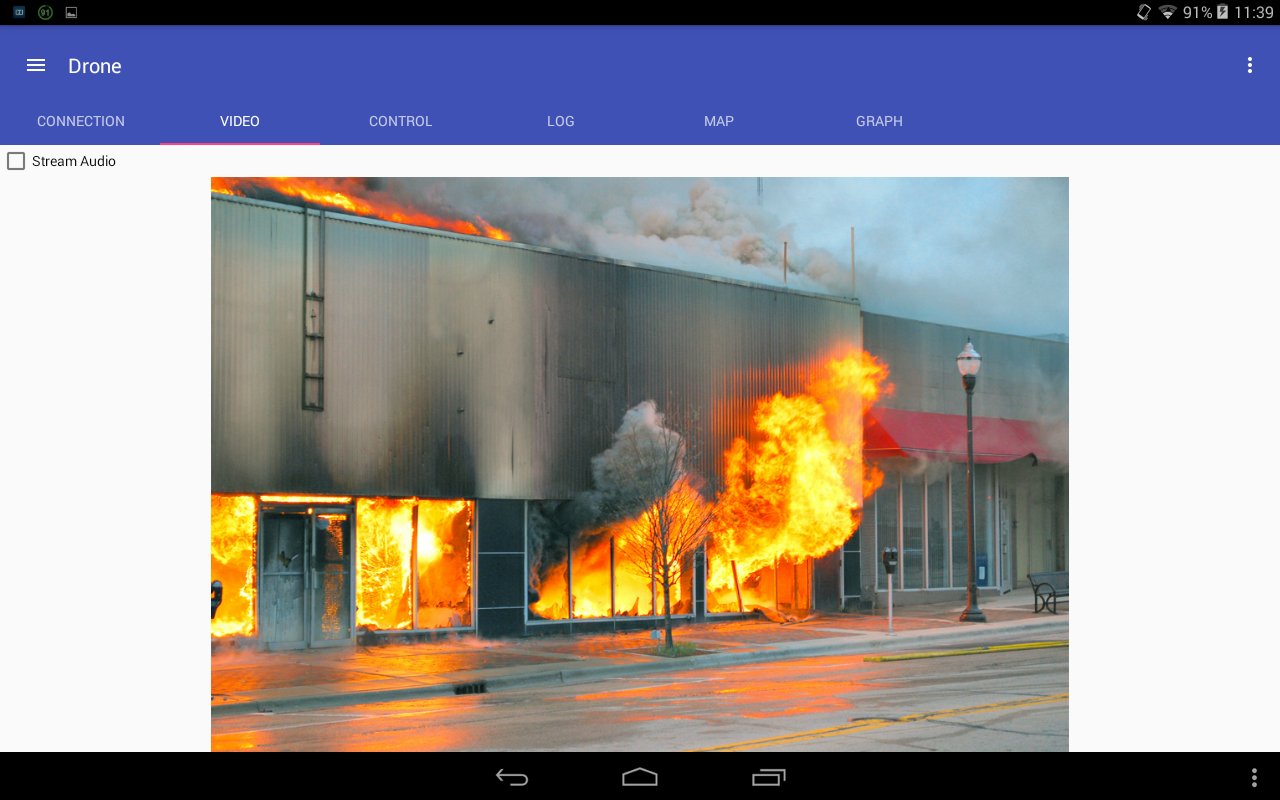
\includegraphics[width=\linewidth]{VideoFragment}
\caption{Video Fragment showing latest image}
\end{subfigure}
\begin{subfigure}[b]{.45\linewidth}
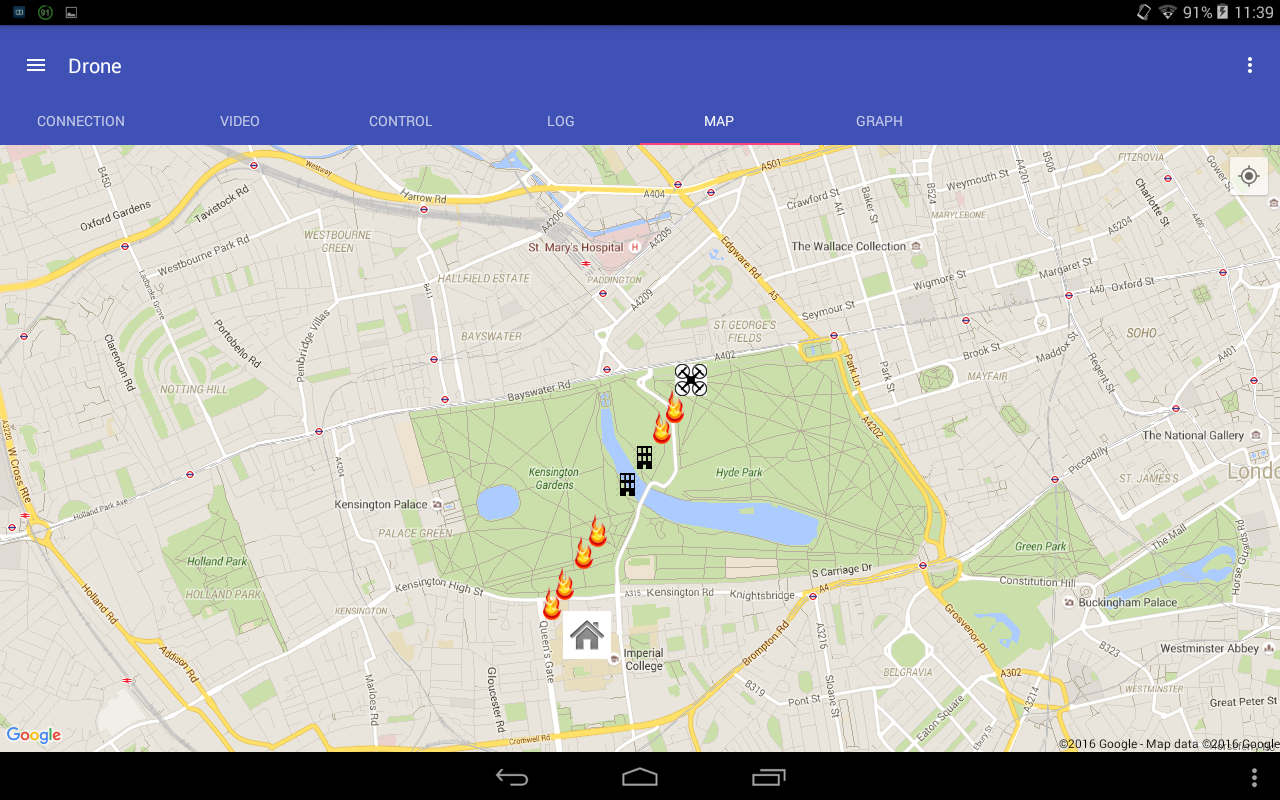
\includegraphics[width=\linewidth]{MapFragment}
\caption{Map Fragment plotting locations of feedback}
\end{subfigure}

\begin{subfigure}[b]{.45\linewidth}
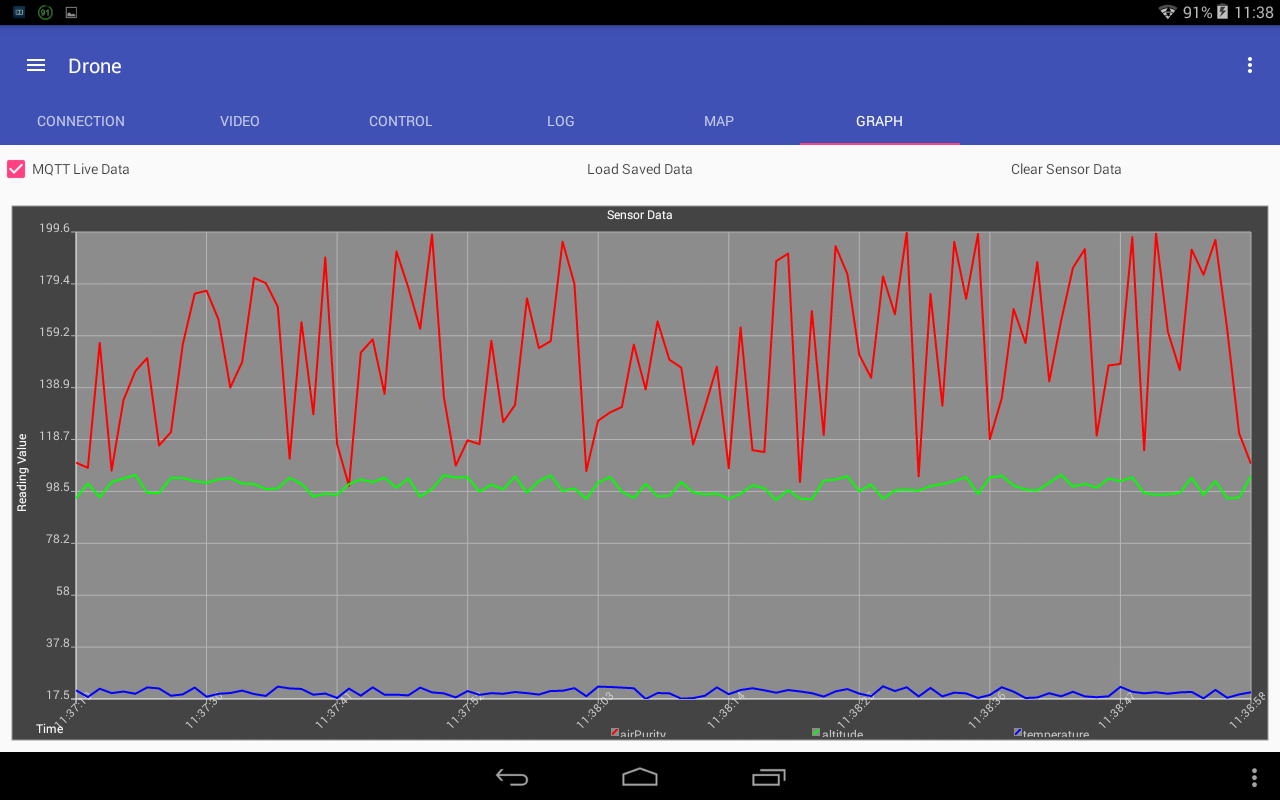
\includegraphics[width=\linewidth]{GraphFragment}
\caption{Graph Fragment, plotting live data}
\end{subfigure}
\begin{subfigure}[b]{.45\linewidth}
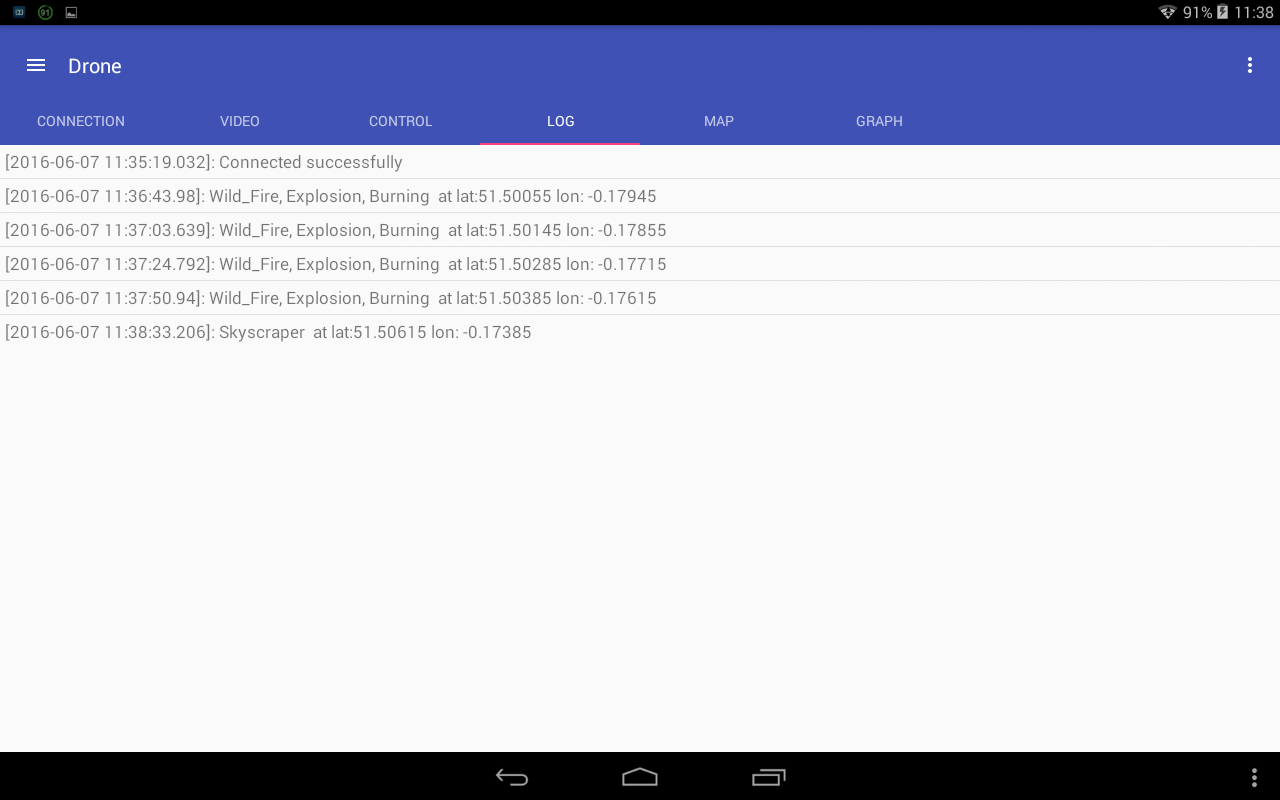
\includegraphics[width=\linewidth]{LogFragment}
\caption{Log Fragment, listing all service feedback}
\end{subfigure}

\end{figure}
\end{landscape}


\subsection{Mocha Testing}
This first code excerpt is a simple example of a Mocha test file, testing API endpoints. A function is defined and run before each test. The tests (`it`) are run sequentially, with the after hook handling cleanup.
\begin{lstlisting} [label=mocha1]
var server = require('../app.js');
function loginAdmin(done){
	request(server)
		.post('/login')
		.auth('jake','pass')
		.expect(200)
		.end(function(err, res){
			if(err){ throw err; }
			cookie = res.headers['set-cookie'].pop().split(';')[0];
			done();
		});
}

describe("Image Endpoints", function() {
	beforeEach(loginAdmin); 	
	var time = new Date().getTime();
	it('GET /api/images should return imageFile list', function(done){
		request(server)
			.get('/api/pixhack/images')
			.set('cookie', cookie)
			.expect('Content-Type', 'application/json; charset=utf-8')
			.expect(200, done);
	});
	it('POST /api/images/:docID should accept valid image', function (done){
	  request(server)
		   .post('/api/pixhack/images/' + time)
		   .send({time:time, location:[50,50]})
		   .attach('image', 'test/sampleFiles/testImage.jpg')
		   .set('cookie', cookie)
		   .expect(200, done)
	});
});

after(function (done) {
	var dirPath = './uploads';
	var files = fs.readdirSync(dirPath);
	if (files.length > 0) {
		for (var i = 0; i < files.length; i++) {
			fs.unlinkSync(dirPath + '/' + files[i]);
		}
	}
	done();
});
\end{lstlisting}

This second excerpt is an example of Scenario testing. `spies` are used to mock object passed in, allowing the interaction with these objects to be investigated. 
\begin{lstlisting}[label=mocha2]

var mqttHandler = {
	sendCommand : sinon.spy(),
	sendEvent: sinon.spy()
};

var sendUpdates = sinon.spy();
var droneName = "testDrone";
var droneCoordinator = new DroneCoordinator(mqttHandler, cloudant, sendUpdates );

function getModeNameWithDelay(callback){
	setTimeout(function(){
		callback(droneCoordinator.getModeName(droneName))
	}, 1100);
}

beforeEach(function(done){
	droneCoordinator.reset(droneName);
	mqttHandler.sendCommand.reset();
	mqttHandler.sendEvent.reset();
	cloudant.db.insert.reset();
	sendUpdates.reset();
	done();
});

describe("Fire", function () {
	beforeEach(function(done){
		IandC.reset();
		mqttHandler.sendCommand.reset();
		done();
	});
	it('should trigger fire mode from image labels', function(done){
            var fire = [{name:"Wild_Fire", score:0.8}, {name:"Rainbow", score:0.53}];
            droneCoordinator.processImageLabels(droneName, fire, new Date().getTime(), [51.5,-0.19]);
            getModeNameWithDelay(  function (result){
                assert.equal(result, "Fire", "Modes do not match");
                assert(mqttHandler.sendCommand.calledTwice, "MQTT Command not sent");
                assert(mqttHandler.sendEvent.calledOnce, "MQTT Event not sent");
                assert(cloudant.db.insert.called, "Database not used");
                assert(sendUpdates.calledWith(droneName, 'event'), "sendUpdates not called correctly");
                done();
            });
        });
});
\end{lstlisting} 


\subsection{Image Recognition Testing}\label{ImageRecTesting}
Table \ref{tab:ImageRecTest} show the confidence values for each returned label for a range of input densities. The set of images used to generate this data were of the head and shoulders of a person sitting in a chair. 
\begin{landscape}
\begin{table}
\caption{Image Recognition Service Confidence For Varying Input Data Density\label{tab:ImageRecTest}}
\begin{tabularx}{\textheight}{|p{2.1cm} X X X X X X X X X X X X X X X X X X X X X|}
\hline
File Name&1&2&3&4&5&6&7&8&9&10&11&12&13&14&15&16&17&18&19&20&21\\ 
\hline
854x480q25&0.64&&&0.83&0.58&0.73&0.74&0.83&0.81&&0.90&&0.95&0.51&0.80&0.71&0.85&&0.59&&0.51\\
854x480q50&0.64&0.83&0.83&&&0.72&0.71&0.84&&&0.90&0.61&0.94&0.51&0.79&0.62&0.84&&0.59&&0.53\\
854x480q75&0.64&&0.83&0.81&&0.73&0.66&0.83&&&0.90&&0.94&0.51&0.77&0.63&0.84&&0.57&&0.52\\
854x480q100&0.64&&0.90&0.82&&0.73&0.60&0.85&&&0.90&&0.94&0.51&0.78&0.57&0.81&&&&\\
1280x720q25&0.64&&0.84&0.84&&0.72&0.63&0.84&&0.50&0.89&&0.89&0.51&0.76&&&&&0.85&\\
1280x720q50&0.64&&0.86&0.79&&0.69&0.54&0.79&&&0.88&&0.89&0.51&0.79&&0.81&0.62&&&\\
1280x720q75&0.64&&0.81&0.83&&0.72&0.51&0.85&&&0.90&&0.89&0.51&0.79&&&0.62&0.50&0.82&\\
1280x720q100&0.64&&0.83&0.84&&0.73&0.53&0.87&0.83&&0.91&&0.90&0.51&0.79&0.55&&&&&\\
1600x900q25&0.64&&0.87&0.82&0.59&0.74&0.52&0.82&&&0.90&&0.89&0.51&0.79&0.50&0.87&&0.53&&0.52\\
1600x900q50&0.64&&0.83&0.80&&0.74&&&0.79&&0.89&&0.89&0.51&0.79&0.63&0.83&0.54&&&\\
1600x900q75&0.64&&0.84&0.82&&0.74&&&0.81&&0.90&&0.89&0.51&0.79&0.56&&0.56&0.50&0.81&\\
1600x900q100&0.64&0.80&&0.83&&0.74&&&0.79&&0.90&&0.87&0.51&0.79&0.55&0.81&0.59&&&\\
1920x1080q25&0.64&&0.86&0.83&0.55&0.72&&&0.84&&0.87&&0.88&0.51&0.79&&0.88&0.54&0.53&&0.51\\
1920x1080q50&0.64&&0.86&0.81&&0.72&0.53&0.76&&&0.89&&0.86&0.51&0.80&0.51&0.79&&&&\\
1920x1080q75&0.64&&0.84&0.82&&0.72&0.57&&&&0.88&&0.88&0.51&0.79&0.54&0.82&&&0.83&\\
1920x1080q100&0.64&0.82&0.77&0.83&&&0.73&&&&0.88&&0.88&0.51&0.79&0.59&0.78&0.59&0.52&&\\
\hline
\end{tabularx}
\end{table}

\begin{table}
\centering
\begin{tabularx}{\textheight}{|c| X |c |X |c |l |}
\hline
Column &  Label & Column & Label & Column & Label\\
\hline
1&Adult& 8 &Dressing Room & 15&Male Adult \\
2&Art Museum & 9 &Escalator & 16 & Pina Colada\\
3&Bathroom &10&Face&17&Rest Room \\
4&Beauty Salon &11&Female Adult &18&Skirt\\
5&Cheese Fondue &12&Food Processor & 19&Sparkling Wine\\
6&Classroom &13&Head and Shoulders & 20&Squash Court\\
7&Concert &14&Individual Person&21&Tea\\
\hline
\end{tabularx}
\end{table}
\end{landscape}

\subsection{Latency Calculator}
The same data as plotted in the Results section, but with an increased Y axis range to show a more complete data set.  
\begin{figure}[h]
\caption{Latency Calculator: Bandwidth Against Latency With Range of File Sizes\label{fig:LatencyVsBandwidthMaxAxis}}
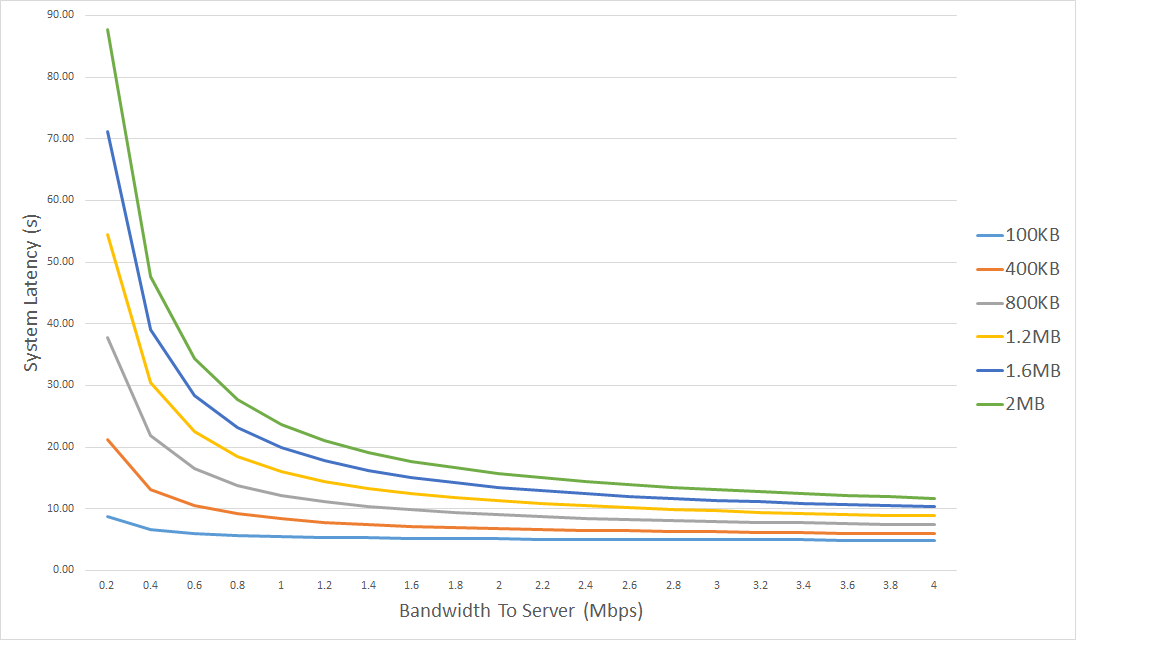
\includegraphics[width=\textwidth]{LatencyVsBandwidthMaxAxis}
\end{figure}











\printbibliography[title={Whole Bibliography}]


\end{document}
